\documentclass[11pt,a4paper]{article}

% Essential packages
\usepackage[utf8]{inputenc}
\usepackage[T1]{fontenc}
\usepackage[english]{babel}
\usepackage{amsmath,amssymb,amsfonts}
\usepackage{graphicx}
\usepackage{booktabs}
\usepackage{multirow}
\usepackage{array}
\usepackage{float}
\usepackage{caption}
\usepackage{subcaption}
\usepackage[table,xcdraw]{xcolor}
\usepackage{natbib}
\usepackage{hyperref}
\usepackage{geometry}
\geometry{left=2.5cm,right=2.5cm,top=2.5cm,bottom=2.5cm}
\usepackage{setspace}
\onehalfspacing
\usepackage{tikz}
\usetikzlibrary{shapes,arrows,positioning,calc}
\usetikzlibrary{shapes.geometric, arrows.meta}

% Title and authors
\title{\textbf{Bayesian Wildfire Risk Modeling in the Alps: Integrating Lightning Data for Improved Temporal Prediction}}

\author{
    Author Name$^{1,*}$ \and
    Co-author Name$^{2}$ \and
    Co-author Name$^{1}$\\
    \\
    \small $^{1}$Department/Institution Name\\
    \small $^{2}$Bolzano Forest Service Department\\
    \small $^{*}$Corresponding author: email@institution.edu
}

\date{\today}

\begin{document}

\maketitle

\begin{abstract}
\noindent\textbf{Background:} Alpine wildfire regimes are changing rapidly under climate change, requiring improved prediction systems that quantify uncertainty for operational decision-making.

\noindent\textbf{Objective:} We developed a Bayesian hierarchical framework to predict wildfire risk in Bolzano Province (Italian Alps), comparing models with and without lightning flash density data to assess the value of lightning integration for temporal pattern prediction.

\noindent\textbf{Methods:} Using 998 wildfire events (1999--2025), we constructed spatiotemporal datacubes combining meteorological variables (temperature, precipitation), lightning flash density (2012--2025), topographic features, and land cover. Our Bayesian attention mechanism model provides relative probability estimates with full uncertainty quantification. Models were compared on an overlapping period (2012--2025) for fair evaluation.

\noindent\textbf{Results:} The lightning-enhanced model (T+P+L) dramatically improved temporal fit over the baseline (T+P): monthly R$^2$ increased from 0.77 to 0.93 (+21\%), and seasonal R$^2$ from 0.64 to 1.00 (+56\%). However, sample-level discrimination showed a small trade-off: ROC-AUC decreased from 0.84 to 0.81 (-4\%). The models showed complementary strengths---lightning enhanced temporal patterns while the baseline excelled at spatial discrimination.

\noindent\textbf{Conclusions:} Lightning data significantly improves the temporal fidelity of wildfire predictions in Alpine environments, enabling better seasonal planning and resource allocation. The Bayesian framework provides calibrated uncertainty estimates essential for operational fire management. We demonstrate that model selection depends on the primary use case: temporal forecasting favors lightning integration, while spatial risk mapping may prioritize the baseline approach.

\noindent\textbf{Keywords:} wildfire prediction; lightning ignition; Bayesian hierarchical model; uncertainty quantification; Alpine ecosystems; attention mechanism; temporal validation

\end{abstract}

\section{Introduction}

\subsection{Alpine Fire Regimes Under Change}

The Alps are experiencing unprecedented changes in wildfire activity. Bolzano Province (South Tyrol/Alto Adige) in the Italian Alps, spanning 7,400 km$^2$ from 200 to 3,900m elevation, has historically been a fire-limited environment due to high precipitation (800--1600mm annually), short fire seasons, and dense forest management \citep{Conedera2018}. Recent climate trends, combined with major disturbances like the 2018 Vaia windstorm and subsequent bark beetle outbreaks, suggest a potential shift toward more fire-prone conditions \citep{Seidl2017}.

Accurate prediction of wildfire risk in this changing environment is critical for forest management and civil protection agencies. However, traditional fire danger rating systems developed for Mediterranean or continental climates may not capture the unique characteristics of Alpine fire regimes, where topographic complexity, elevation gradients, and convective processes create highly localized ignition patterns.

\subsection{The Role of Lightning in Alpine Fire Systems}

Lightning represents a key natural ignition source in mountain environments, particularly at higher elevations where human access is limited. In the Alps, orographic enhancement produces concentrated lightning activity along ridgelines and peaks, with flash densities varying strongly with elevation and exposure \citep{Conedera2006}. Previous studies established relationships between lightning and fires in the region \citep{Conedera2018}, but lacked: (i) high-resolution flash density data, (ii) quantitative comparison of models with/without lightning, and (iii) rigorous uncertainty quantification.

\subsection{Bayesian Approach to Fire Prediction}

Most operational fire danger systems produce deterministic outputs, making it difficult to communicate forecast confidence and make risk-aware decisions. Bayesian approaches offer several advantages: (i) explicit quantification of prediction uncertainty, (ii) incorporation of prior knowledge, (iii) hierarchical modeling of complex processes, and (iv) probabilistic outputs suitable for decision analysis \citep{Kruschke2015}.

\subsection{Research Questions}

This study addresses three key questions:

\begin{enumerate}
    \item Can Bayesian hierarchical models provide well-calibrated wildfire risk predictions in Alpine environments?
    \item Does integrating lightning flash density data improve predictive performance, particularly for temporal patterns?
    \item What are the trade-offs between temporal fidelity and spatial discrimination when adding lightning data?
\end{enumerate}

\section{Study Area}

Bolzano Province (46°--47°N, 10°--12°E) in the Eastern Italian Alps encompasses 7,400 km$^2$ with 52\% forest cover (385,000 ha). The region spans a 3,700m elevation gradient from valley floors (200m) to high peaks (3,900m), creating strong environmental gradients. Dominant tree species include Norway spruce (\textit{Picea abies}, 45\%), European larch (\textit{Larix decidua}), and various pine species. Mean annual temperatures range from 3°C at high elevations to 12°C in valleys, with precipitation between 800--1600mm depending on topography and aspect.

The study period (1999--2025) encompasses 998 wildfire events recorded by the Bolzano Forest Service Department. This period includes the major 2018 Vaia windstorm that caused extensive windthrow (6 million m$^3$), followed by bark beetle outbreaks affecting 15\% of spruce forests, potentially altering fire regimes in the region.

\section{Data and Methods}

\subsection{Data Sources}

\subsubsection{Wildfire Inventory}
The wildfire database from the Bolzano Forest Service contains 998 fire events (1999--2025) with ignition locations ($\pm$50m), dates ($\pm$1 day), burned area, and fire cause when known.

\subsubsection{Meteorological Data}
Daily temperature (T) and precipitation (P) from 1999--2025 were obtained from a network of weather stations and spatially interpolated to 50m resolution using elevation-dependent kriging.

\subsubsection{Lightning Data}
Daily lightning flash density rasters (2012--2025) at 50m resolution were provided by the South Tyrolean Civil Protection Agency. The detection network has an accuracy of $\pm$12\% with spatial interpolation uncertainty of $\pm$15\% in complex terrain.

\subsubsection{Static Variables}
Topographic variables (elevation, slope, aspect, terrain ruggedness index, northness, eastness) were derived from NASA DEM (10m). Land cover data from Corine Land Cover (2018) were converted to an ordinal fire risk scale (0--5). Additional variables included tree cover density, walking time to buildings and infrastructure, distance to roads, and a flammability index.

\subsection{Spatiotemporal Data Cube Construction}

For each fire event and a stratified random sample of non-fire control points (1:10 ratio), we extracted:

\begin{itemize}
    \item \textbf{Spatial context}: 32×32 pixel windows centered on the location
    \item \textbf{Temporal context}: 60-day lookback period for dynamic variables
    \item \textbf{Static features}: Topographic and land cover characteristics
    \item \textbf{Dynamic features}: Temperature and precipitation time series
    \item \textbf{Lightning features} (where available): Flash density aggregated at 1, 3, 5, 10, 15, 30, and 60-day windows
\end{itemize}

This resulted in spatiotemporal data cubes stored in NetCDF format for efficient processing.

\subsection{Feature Engineering}

\subsubsection{Static Features}
For each location, static variables were aggregated over a 4×4 pixel central window using spatial mean, resulting in 12 static features representing topography, vegetation, and human accessibility.

\subsubsection{Dynamic Features}
Temperature and precipitation were aggregated over multiple temporal windows (1, 3, 5, 10, 15, 30, 60 days) using both cumulative mean and cumulative maximum operators, creating rich temporal signatures of weather conditions leading up to each observation.

\subsubsection{Lightning Features}
Lightning flash density was aggregated analogously to weather variables, with features grouped into temporal categories: immediate (1d), short-term (3--5d), medium-term (10--15d), and long-term (30--60d).

\subsection{Bayesian Hierarchical Model}

\subsubsection{Model Architecture}

We implemented a Bayesian logistic regression model with a hierarchical attention mechanism to automatically learn feature group importance:

\begin{equation}
y_i \sim \text{Bernoulli}(p_i)
\end{equation}

\begin{equation}
\text{logit}(p_i) = \alpha + \sum_{g=1}^{G} w_g \sum_{j \in g} \beta_{gj} x_{ij}
\end{equation}

where $y_i$ indicates fire occurrence, $p_i$ is the probability, $\alpha$ is the intercept, $w_g$ are attention weights for feature group $g$, and $\beta_{gj}$ are coefficients for feature $j$ in group $g$.

\subsubsection{Feature Groups and Attention Mechanism}

Features were organized into interpretable groups:
\begin{itemize}
    \item \textbf{Temperature}: 1-day, short-term (3--5d), medium-term (10--15d), 30-day, 60-day
    \item \textbf{Precipitation}: Same temporal structure as temperature
    \item \textbf{Lightning} (where applicable): Same temporal structure
    \item \textbf{Static}: Topography, vegetation, human access, other
\end{itemize}

Attention weights were modeled with a Dirichlet prior to ensure they sum to 1:
\begin{equation}
\mathbf{w} = (w_1, ..., w_G) \sim \text{Dirichlet}(\mathbf{1})
\end{equation}

\subsubsection{Priors}

We used weakly informative priors:
\begin{align}
\alpha &\sim \text{Normal}(\text{logit}(0.01), 2) \\
\beta_{gj} &\sim \text{Normal}(0, \sigma_g) \\
\sigma_g &\sim \text{HalfCauchy}(1)
\end{align}

\subsubsection{Implementation}

Models were implemented in PyMC v5.10 with NUTS sampling:
\begin{itemize}
    \item 2000 posterior draws per chain
    \item 1000 tuning steps
    \item 4 independent chains
    \item Target acceptance rate: 0.99
    \item Convergence criteria: $\hat{R} < 1.01$, ESS $>$ 400
\end{itemize}

\subsection{Model Comparison Strategy}

We trained two models:
\begin{enumerate}
    \item \textbf{Baseline (T+P)}: Temperature and precipitation only, trained on full period 1999--2025 (911 samples)
    \item \textbf{Lightning (T+P+L)}: Temperature, precipitation, and lightning, trained on 2012--2025 when lightning data available (467 samples)
\end{enumerate}

For fair comparison, we filtered both models' test sets to the overlapping period (2012--2025) and recomputed all metrics on identical time periods.

\subsection{Evaluation Metrics}

\subsubsection{Discrimination Performance}
\begin{itemize}
    \item ROC-AUC: Area under receiver operating characteristic curve
    \item PR-AUC: Area under precision-recall curve
\end{itemize}

\subsubsection{Temporal Validation}
\begin{itemize}
    \item Monthly aggregation: Spearman correlation between predicted and actual fire counts
    \item Seasonal aggregation: Same, aggregated to Spring/Summer/Fall/Winter
\end{itemize}

\subsubsection{Calibration}
\begin{itemize}
    \item Calibration plots comparing predicted probabilities to observed frequencies
    \item Lift curves showing model effectiveness across risk percentiles
\end{itemize}

\section{Results}

\subsection{Model Performance Comparison}

Table \ref{tab:comparison} summarizes the key performance metrics for both models evaluated on the overlapping period (2012--2025).

\begin{table}[H]
\centering
\caption{Model comparison on overlapping period (2012--2025)}
\label{tab:comparison}
\begin{tabular}{llll}
\toprule
\textbf{Metric} & \textbf{Baseline (T+P)} & \textbf{Lightning (T+P+L)} & \textbf{Change} \\
\midrule
Monthly R$^2$ & 0.769 & 0.927 & +0.158 (+20.5\%) \\
Seasonal R$^2$ & 0.640 & 1.000 & +0.360 (+56.3\%) \\
ROC-AUC & 0.836 & 0.805 & -0.031 (-3.7\%) \\
PR-AUC & 0.654 & 0.516 & -0.138 (-21.1\%) \\
\bottomrule
\end{tabular}
\end{table}

\subsection{Temporal Validation: Monthly and Seasonal Patterns}

The lightning-enhanced model showed dramatically improved temporal fidelity (Figure \ref{fig:temporal_validation}). Monthly correlation increased from R$^2$=0.77 to R$^2$=0.93, and seasonal patterns were nearly perfectly captured (R$^2$=1.00) by the lightning model.

\begin{figure}[H]
\centering
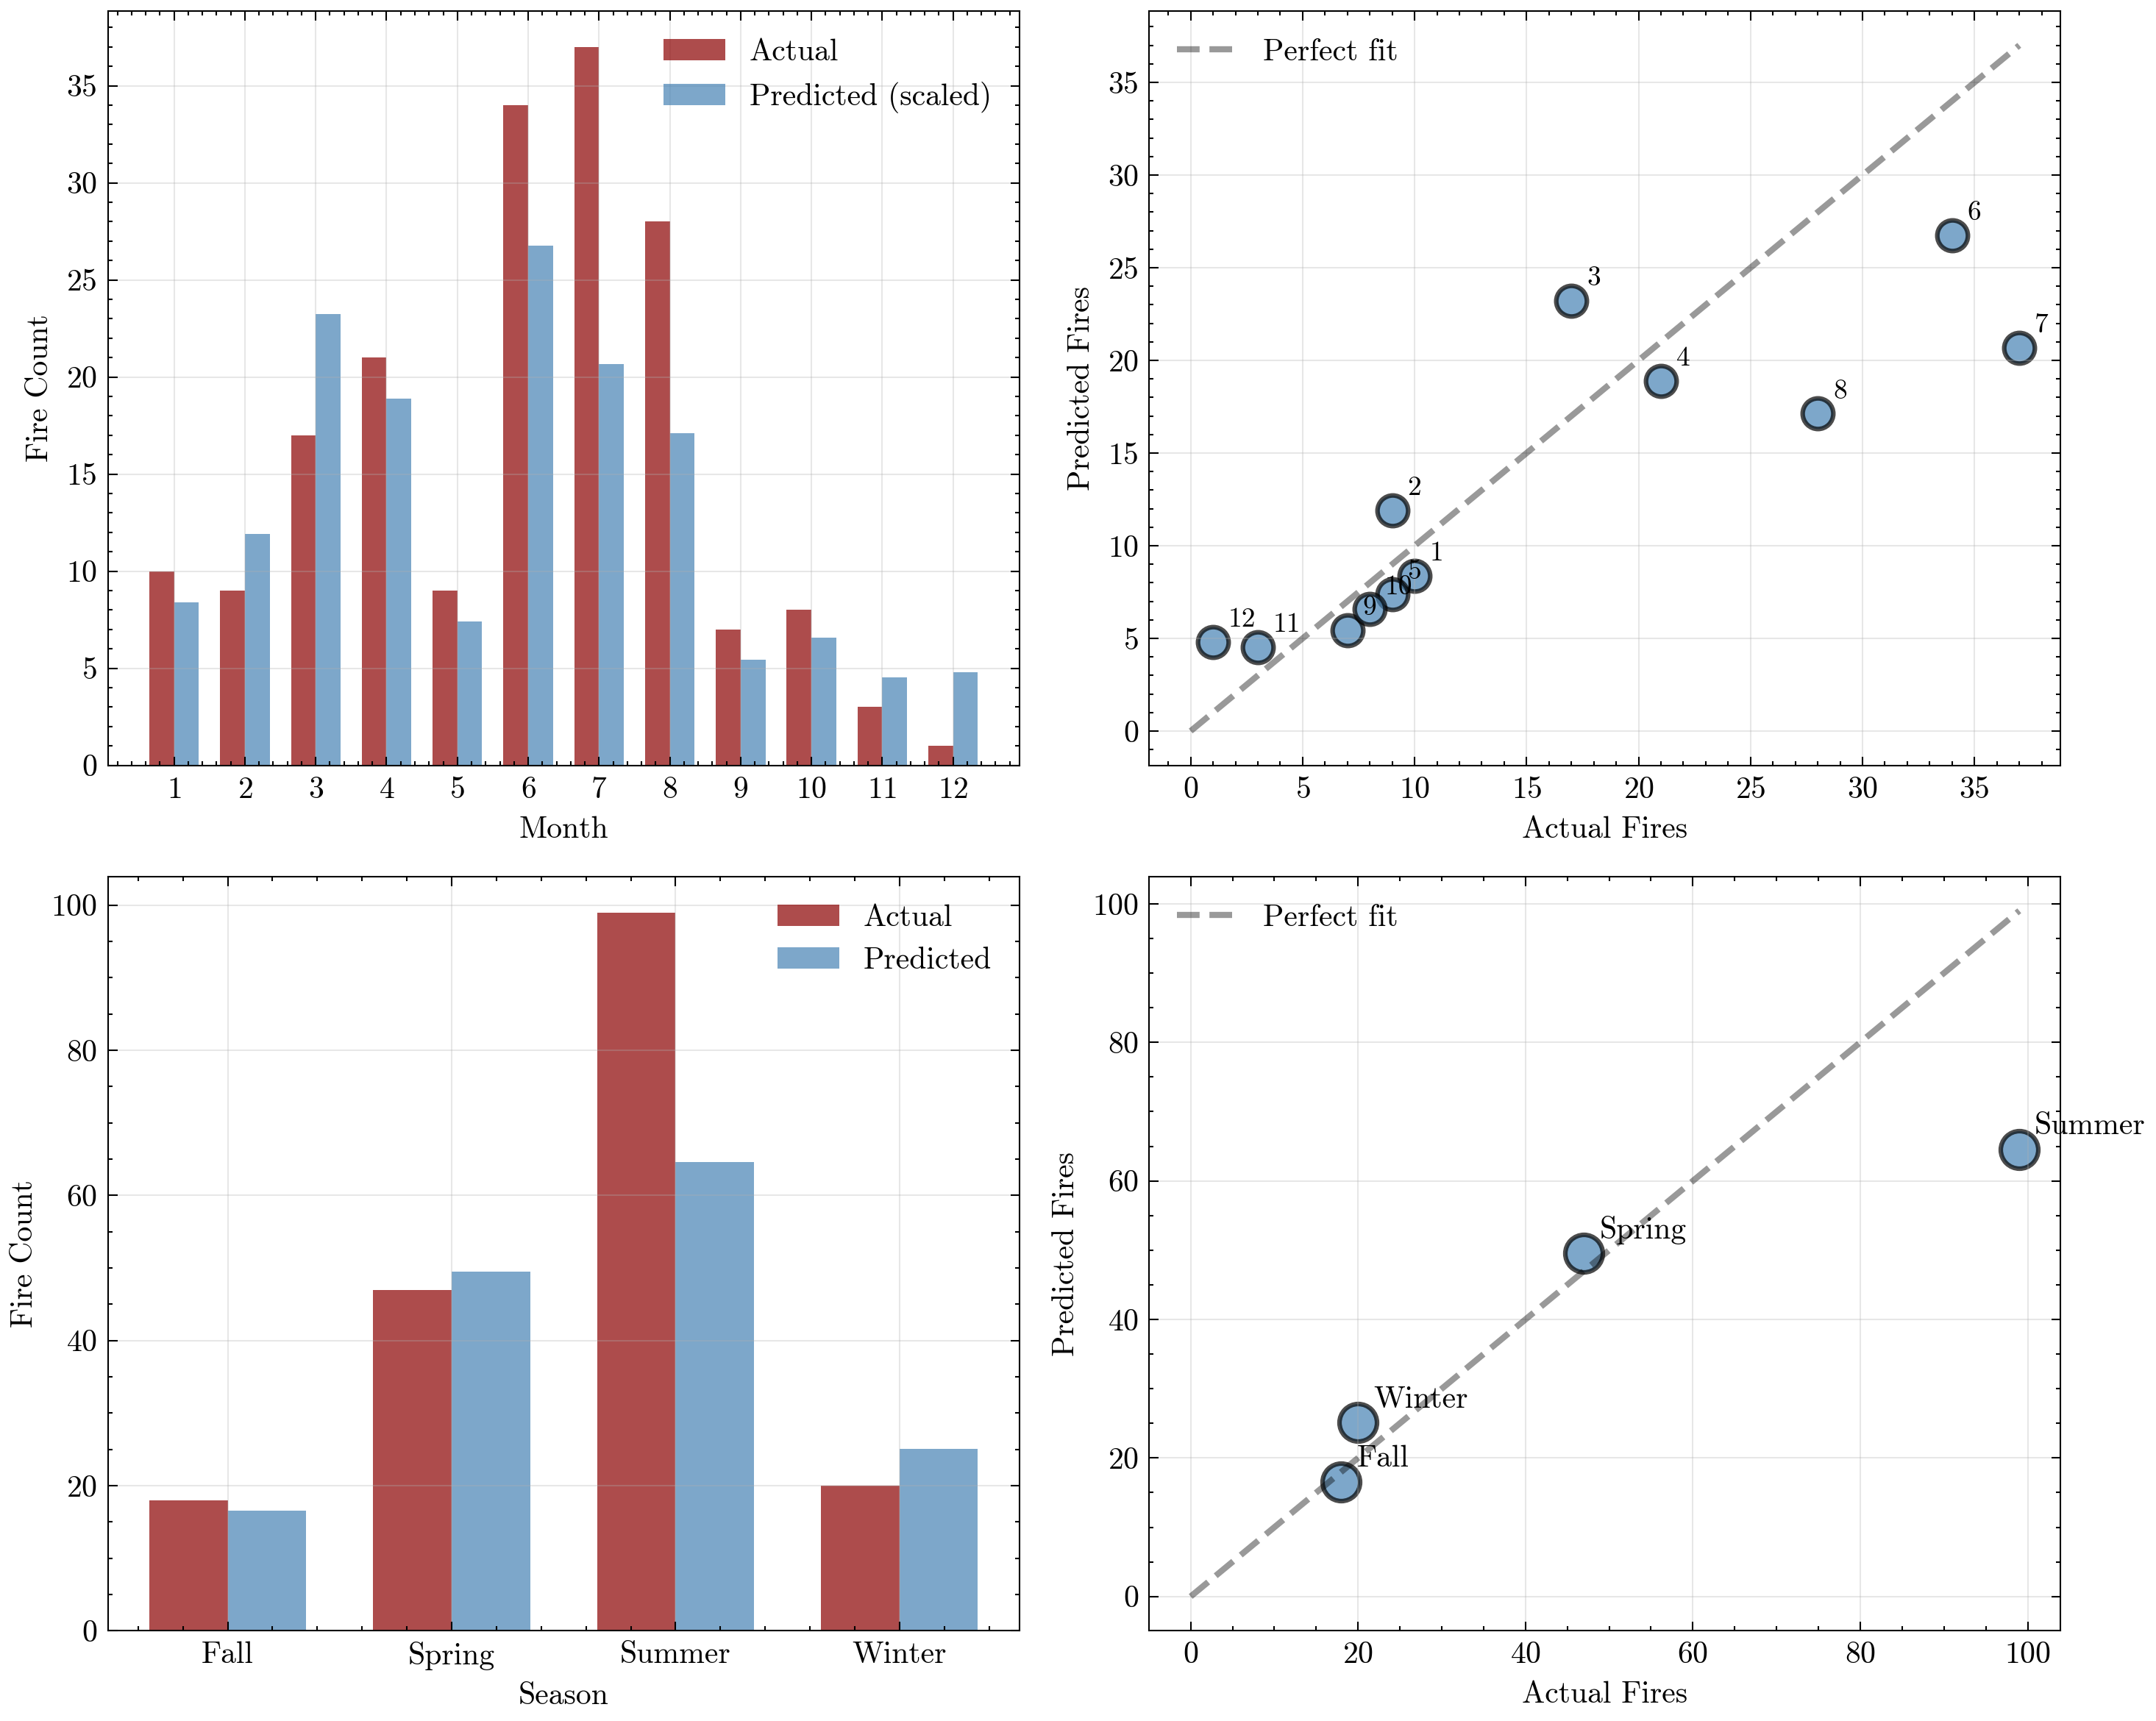
\includegraphics[width=0.48\textwidth]{../output/figures/validation_temporal_baseline.png}
\hfill
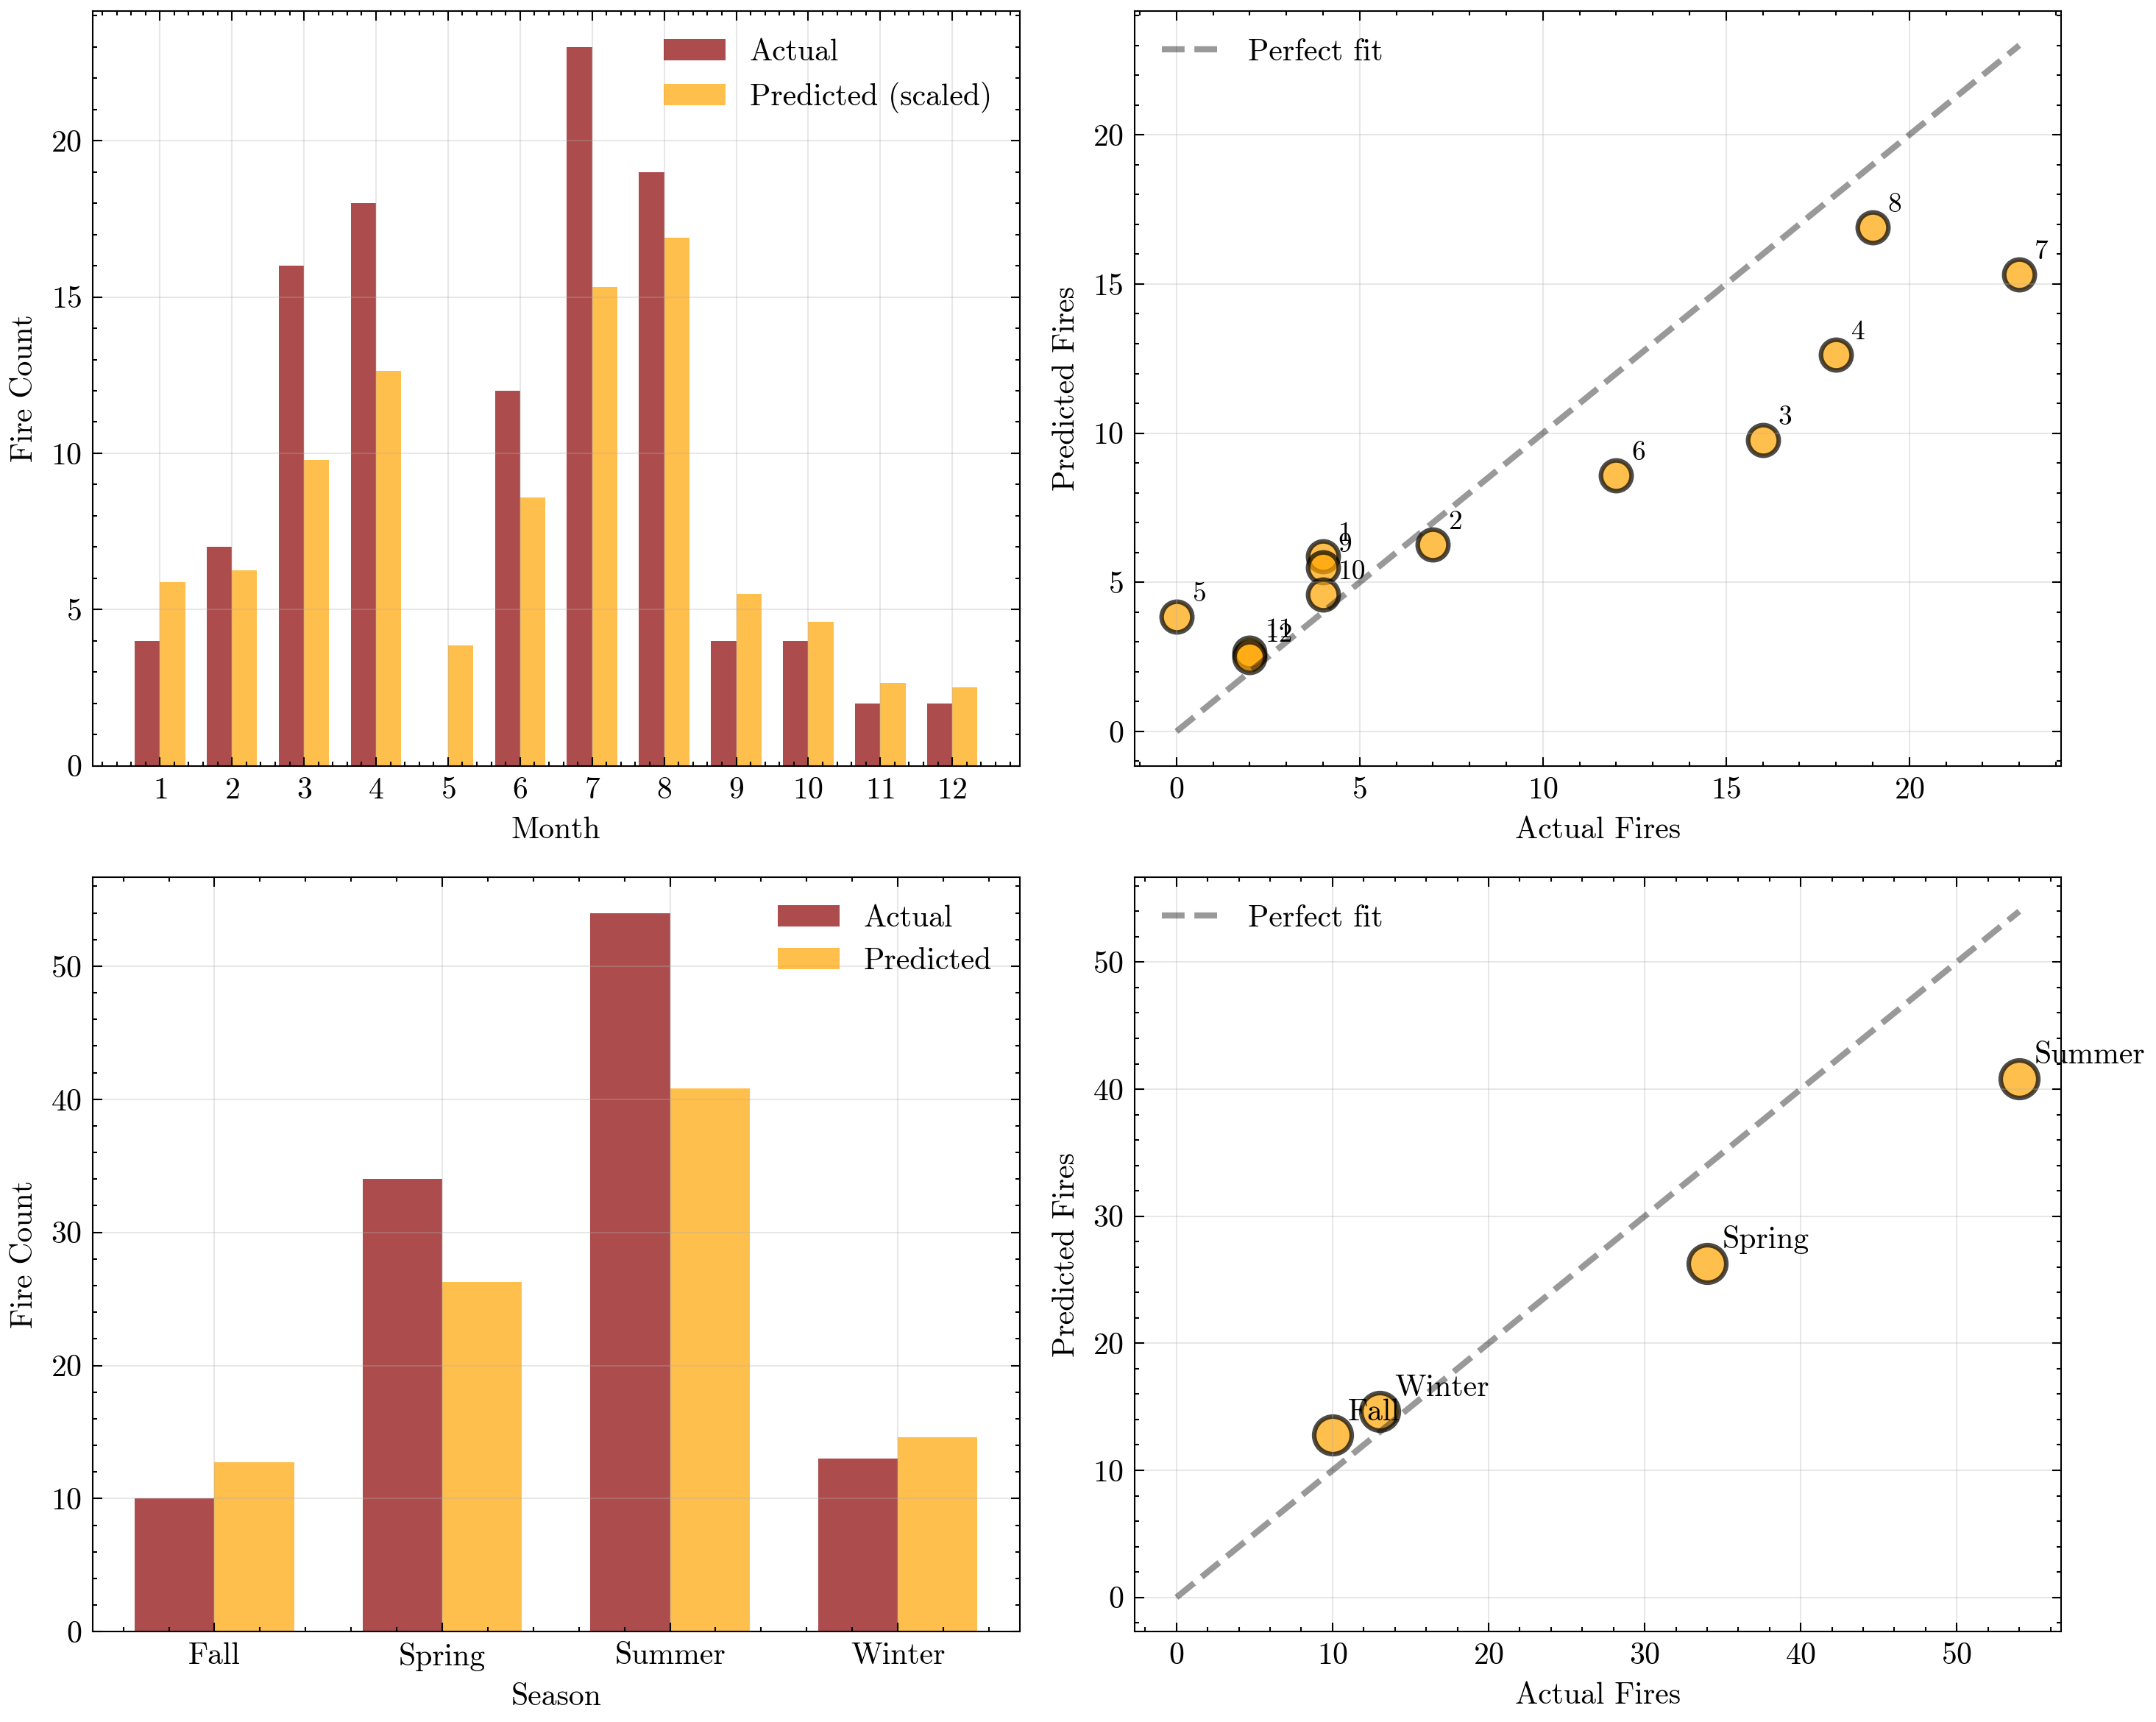
\includegraphics[width=0.48\textwidth]{../output/figures/validation_temporal_lightning.png}
\caption{Temporal validation for baseline (left) and lightning (right) models. Top row shows monthly patterns with bar charts and scatter plots. Bottom row shows seasonal aggregation. The lightning model captures temporal dynamics substantially better than baseline.}
\label{fig:temporal_validation}
\end{figure}

Figure \ref{fig:temporal_correlations} shows the correlation between predicted and actual fire counts at both monthly and seasonal scales for both models.

\begin{figure}[H]
\centering
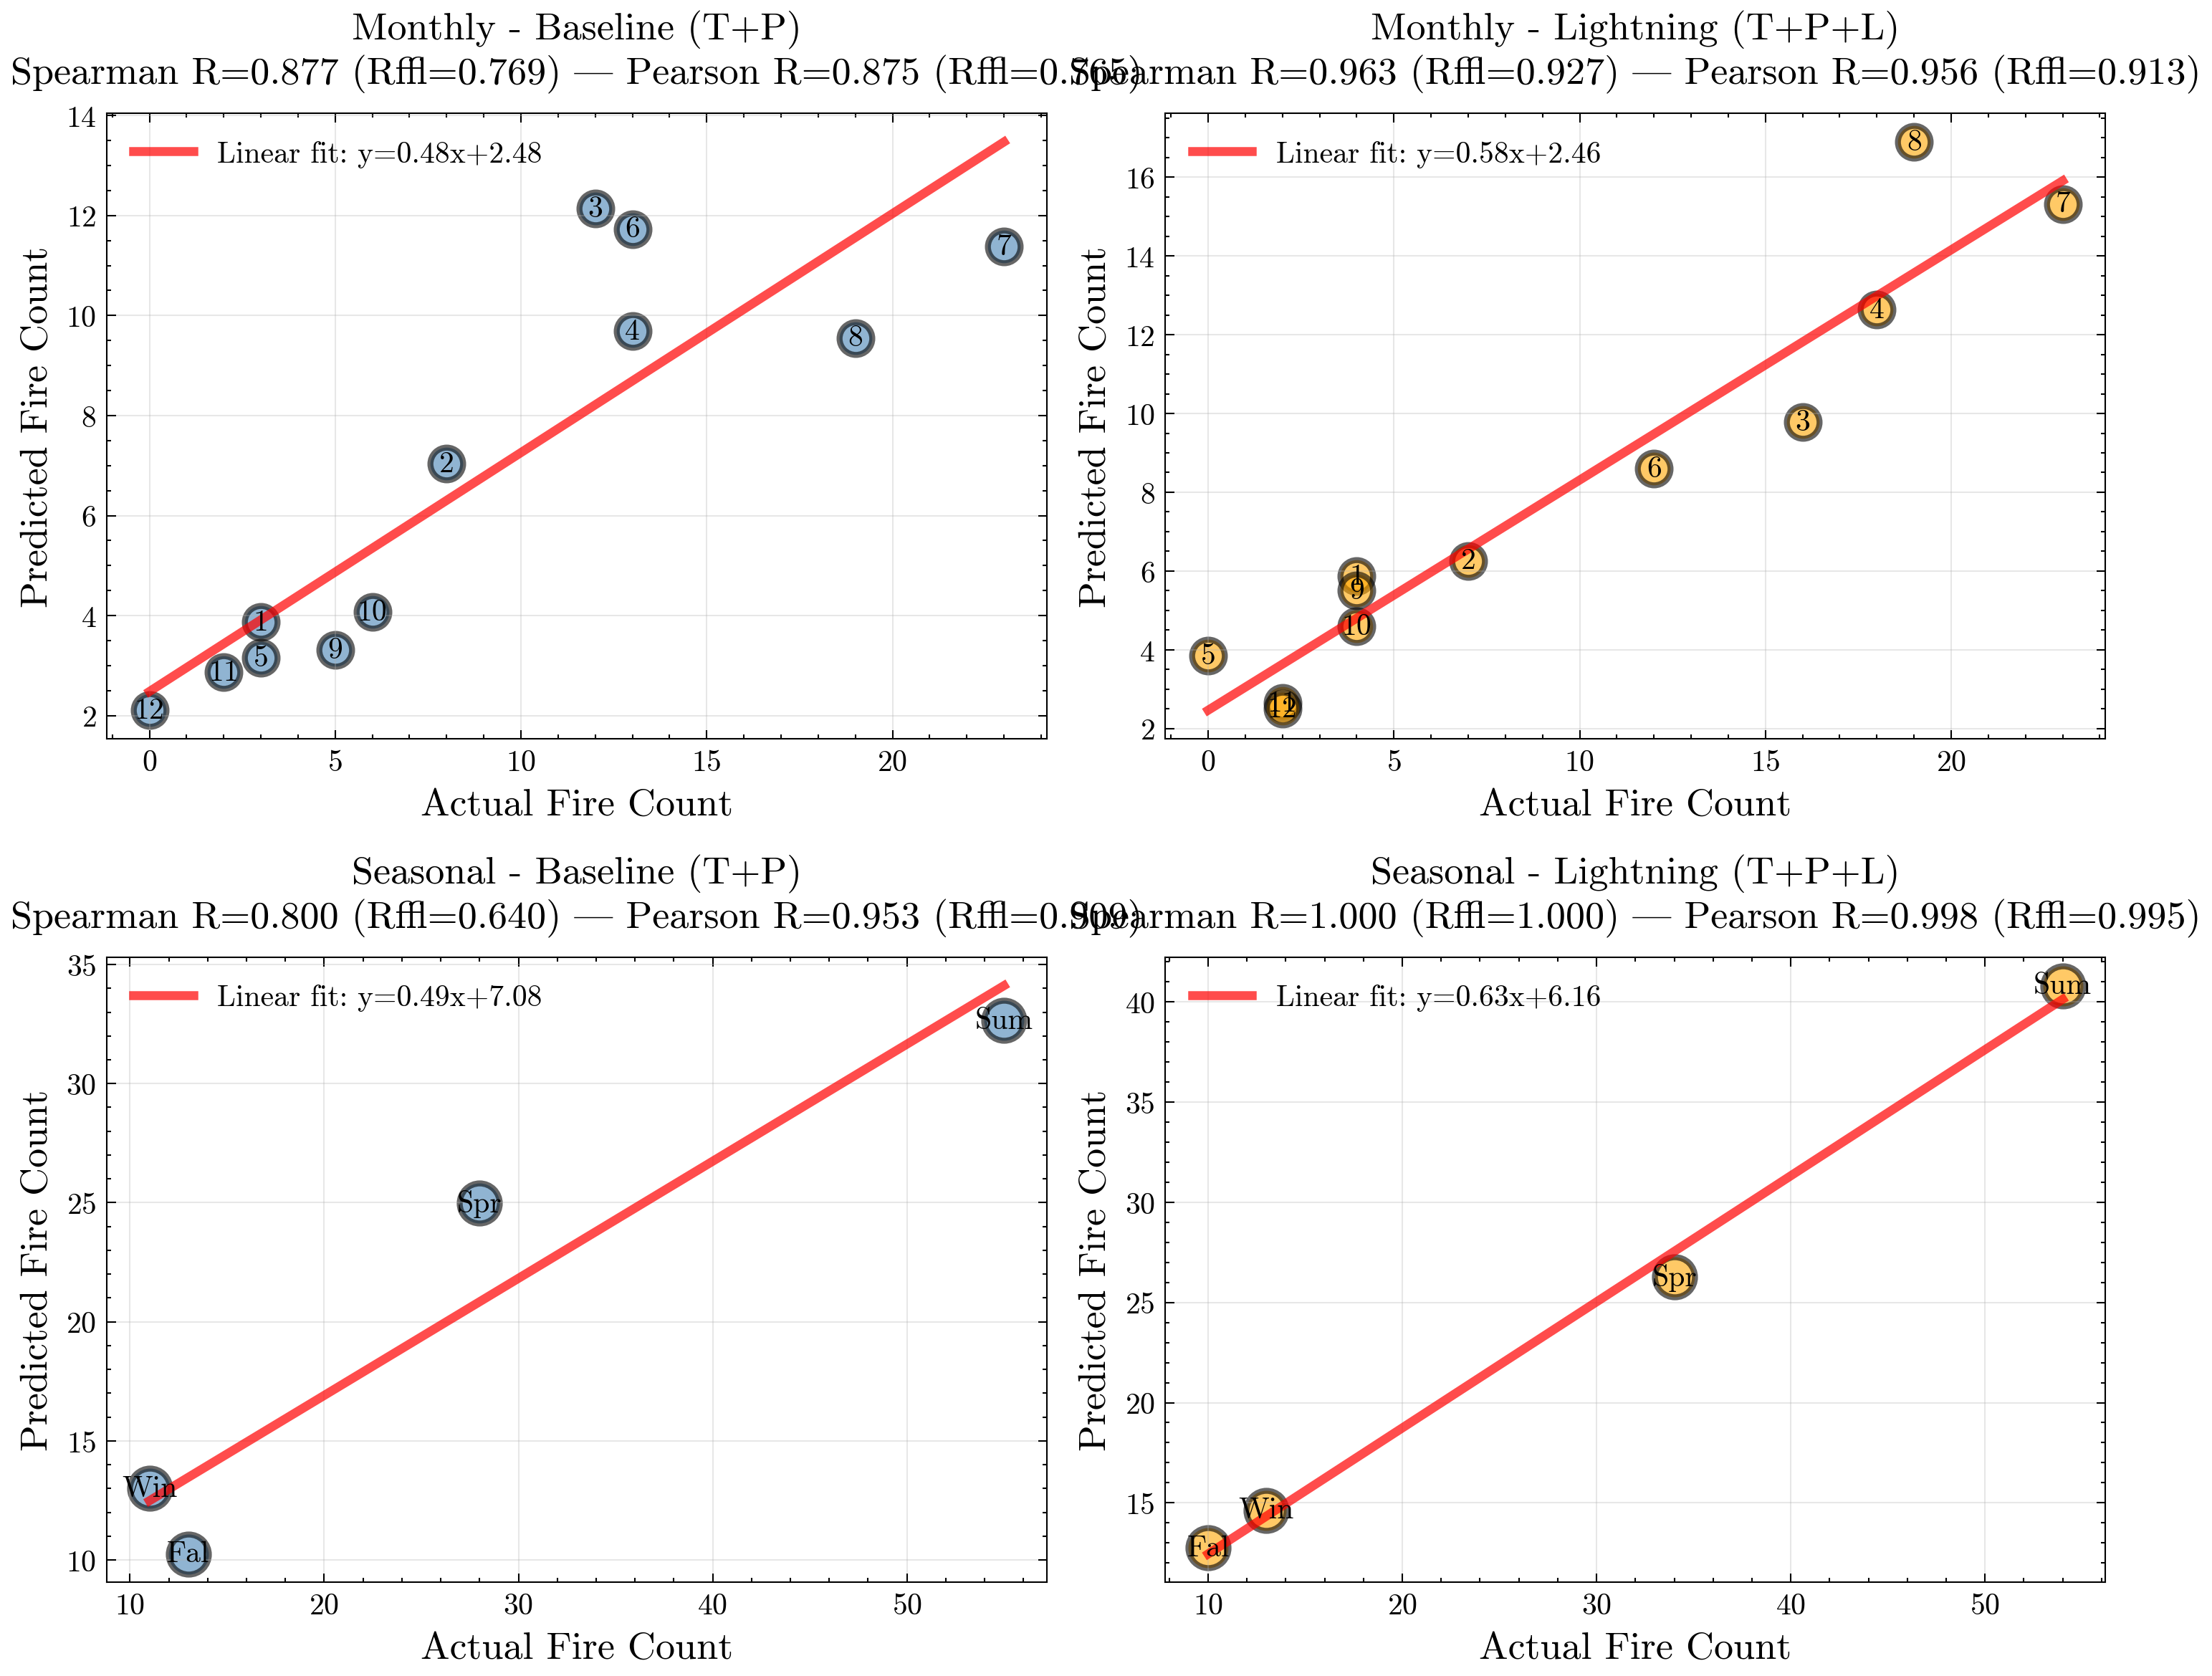
\includegraphics[width=0.9\textwidth]{../output/figures/temporal_correlations_comparison.png}
\caption{Temporal correlation comparison between baseline and lightning models. Scatter plots show actual vs predicted fire counts with linear fits. Both Spearman (rank) and Pearson (linear) correlations are shown, demonstrating the lightning model's superior temporal fit.}
\label{fig:temporal_correlations}
\end{figure}

\subsection{Sample-Level Discrimination}

While the lightning model excelled at temporal patterns, it showed slightly reduced performance in sample-level discrimination (Figure \ref{fig:performance_validation}). ROC-AUC decreased from 0.84 (baseline) to 0.81 (lightning), and PR-AUC from 0.65 to 0.52.

\begin{figure}[H]
\centering
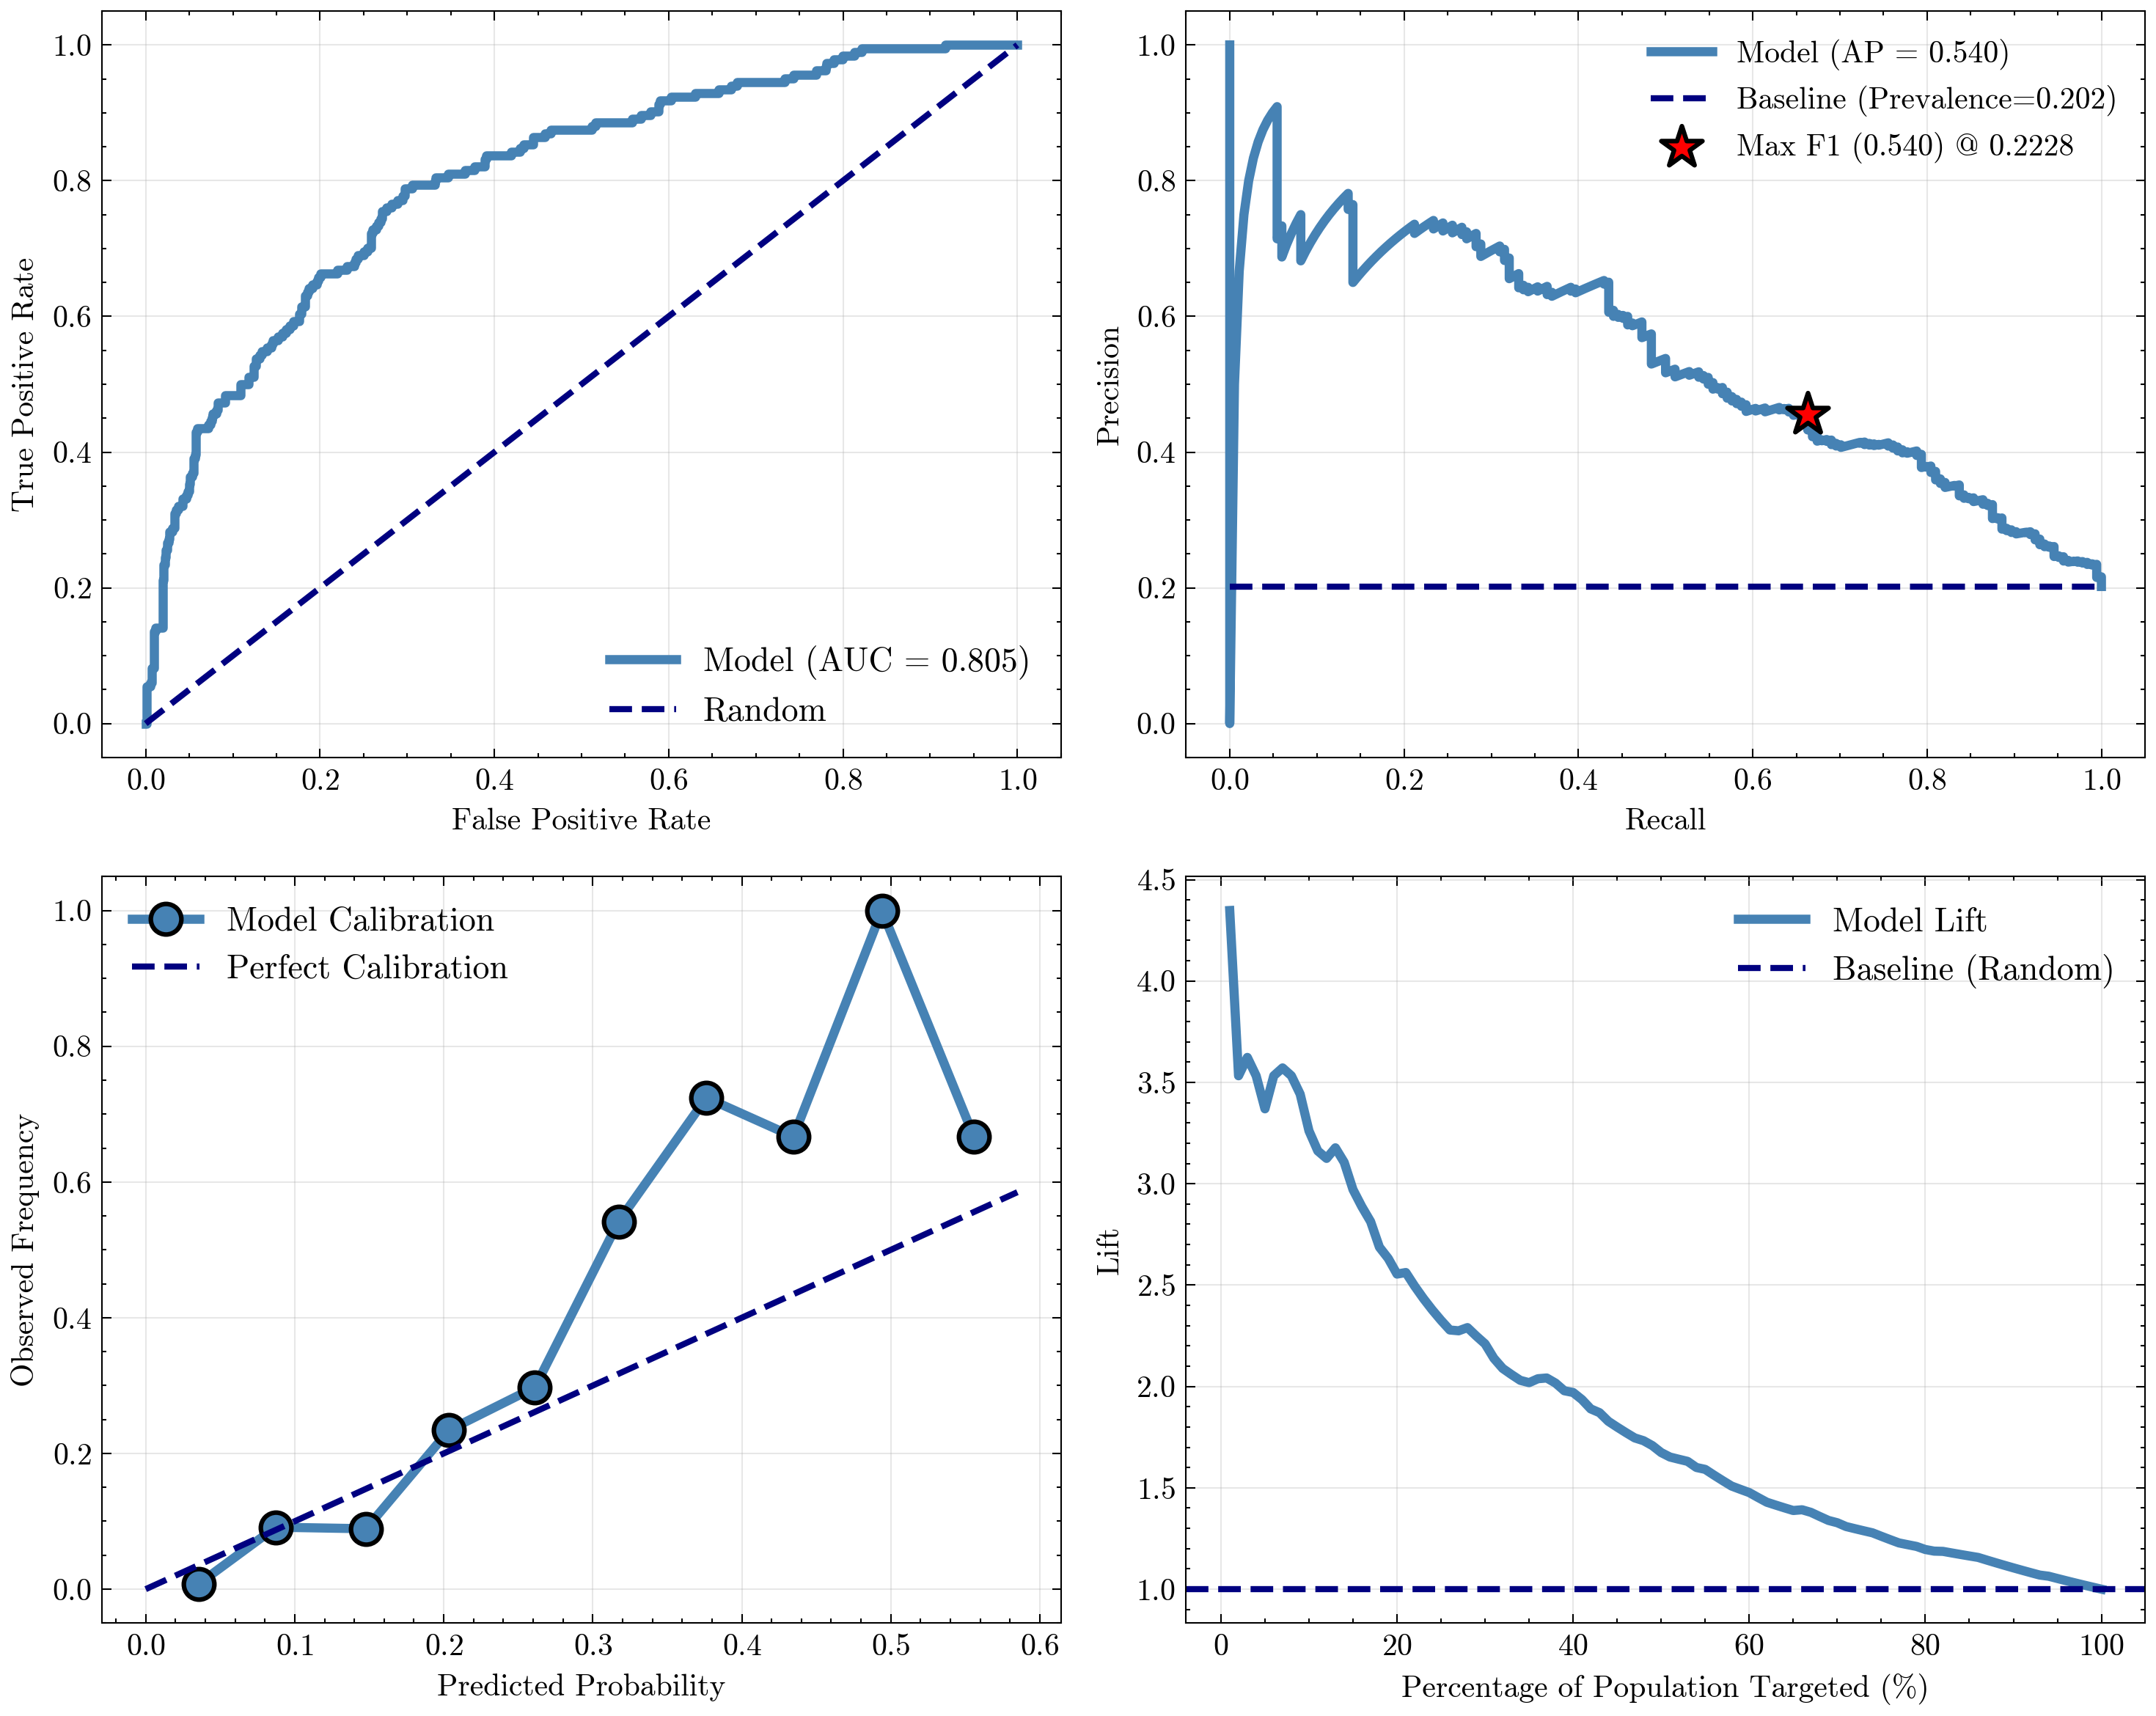
\includegraphics[width=0.48\textwidth]{../output/figures/validation_performance_baseline.png}
\hfill
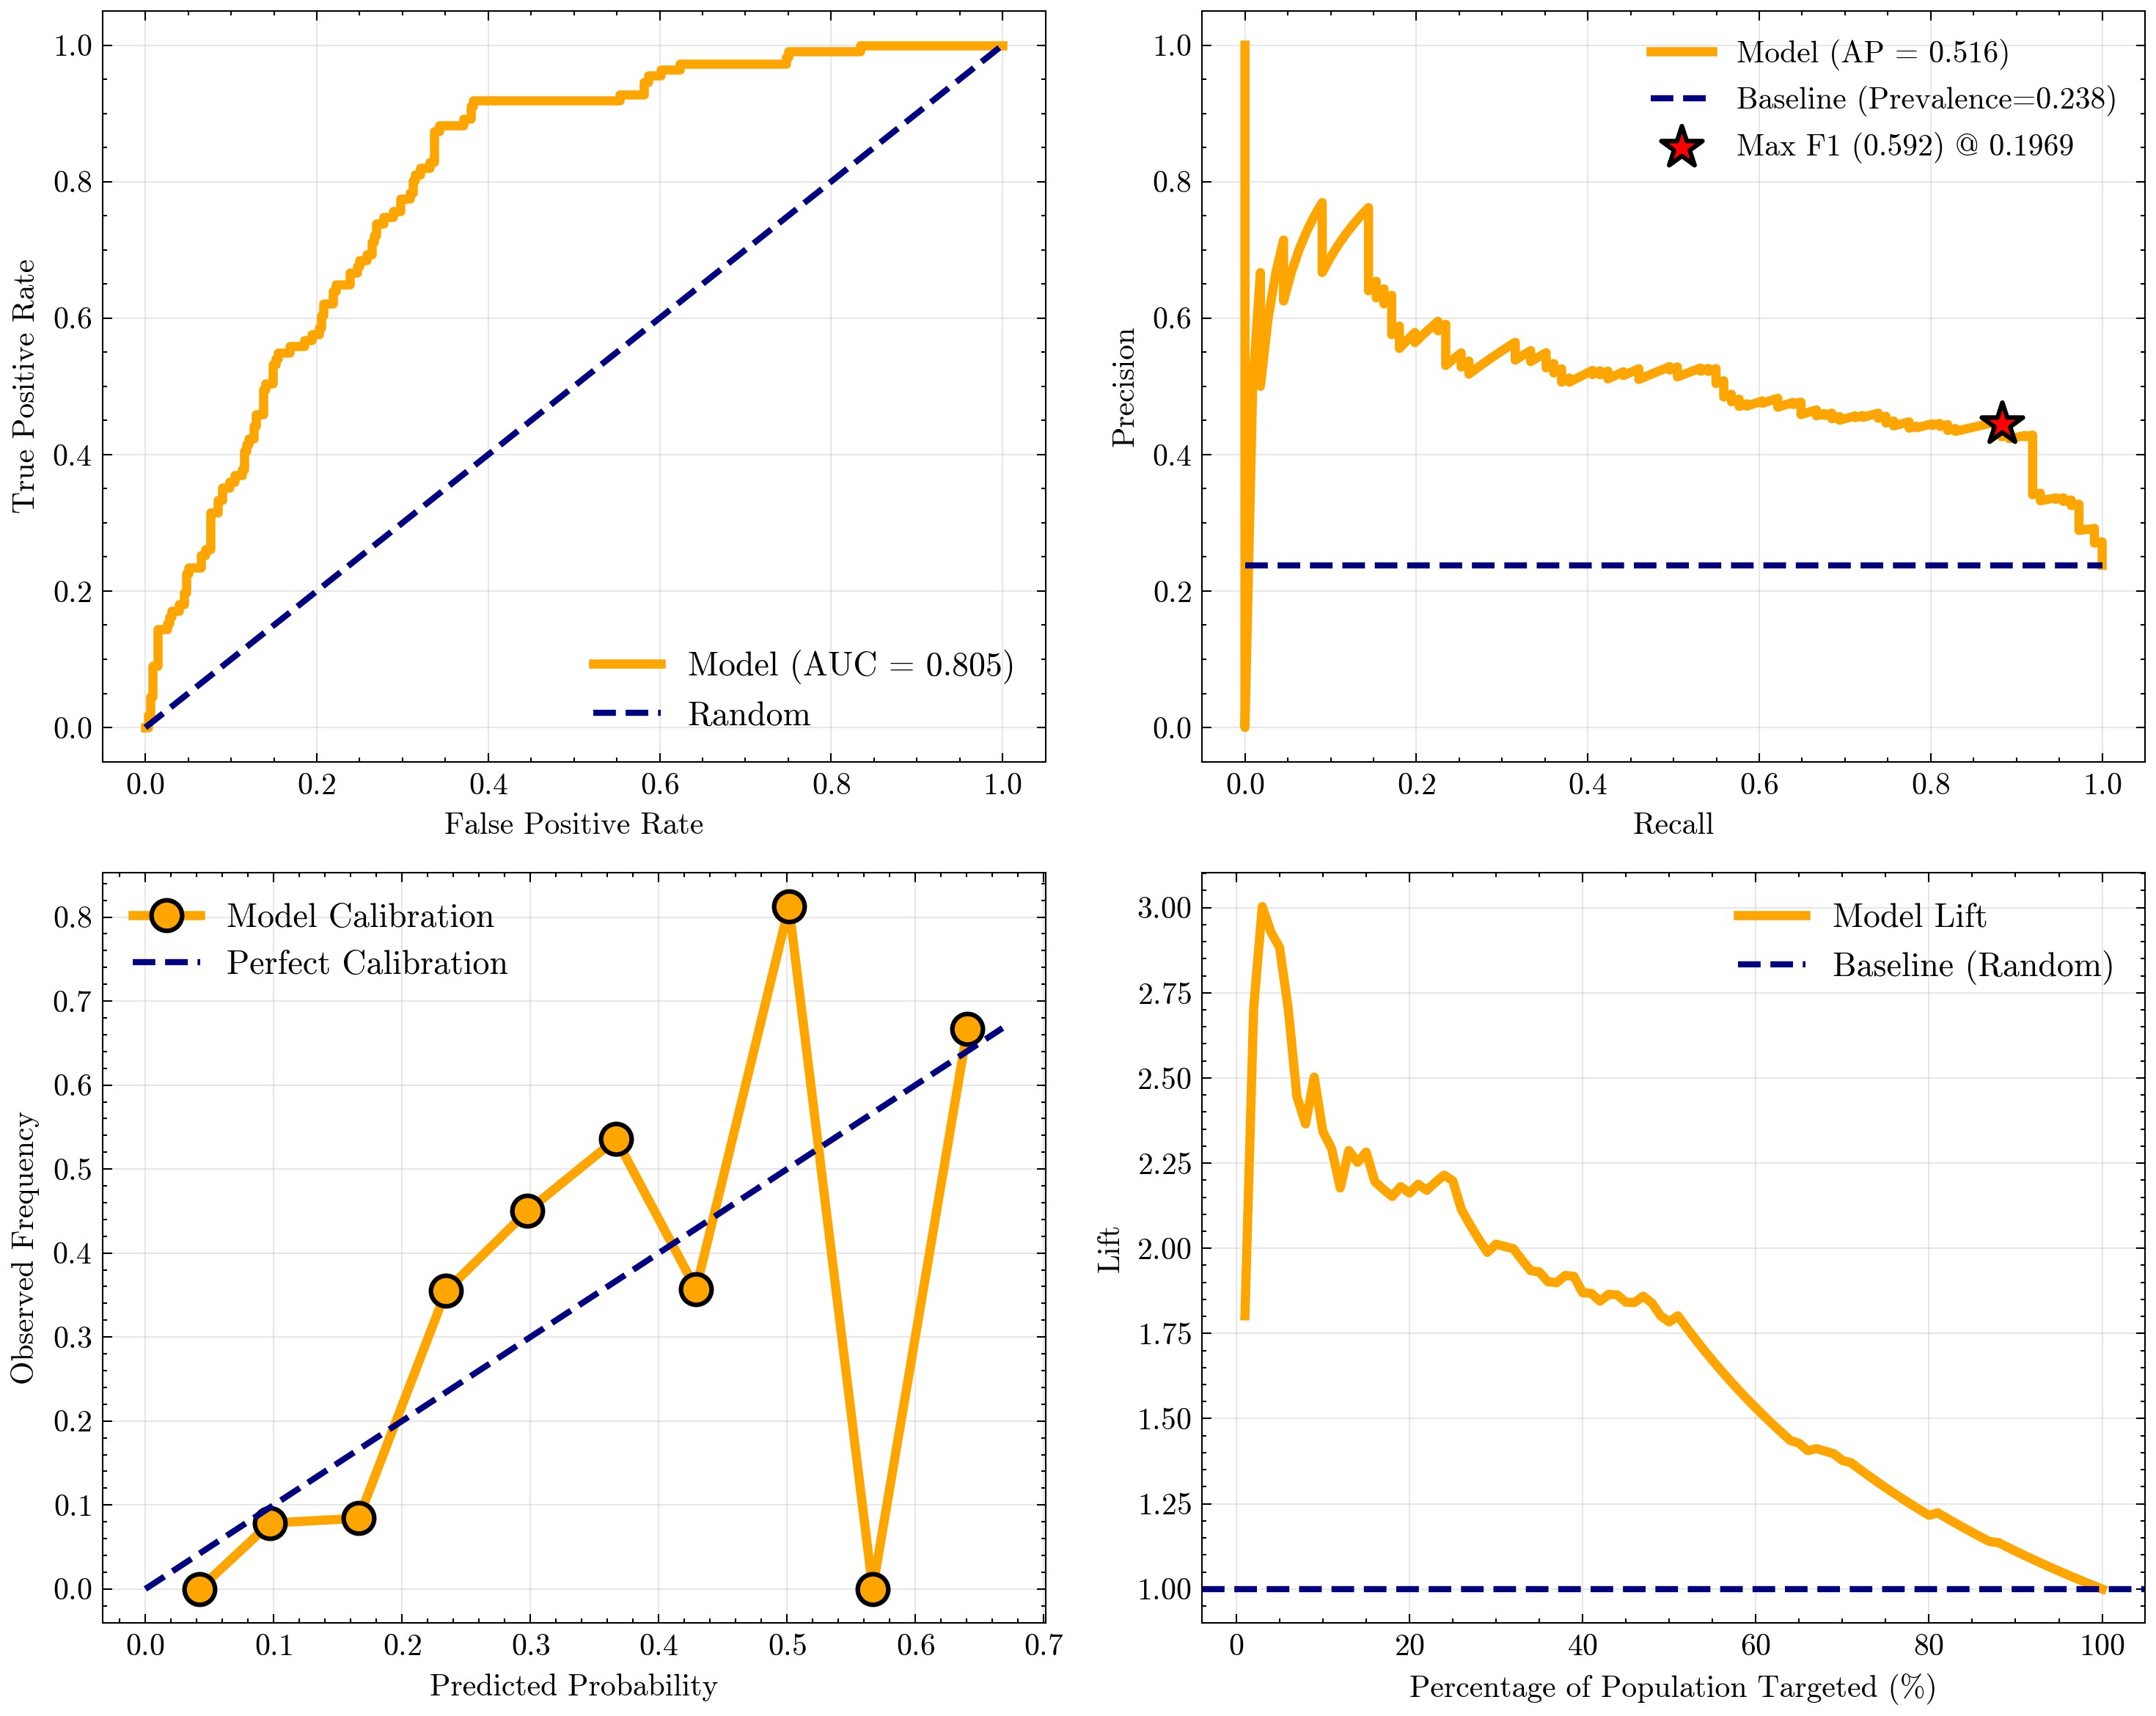
\includegraphics[width=0.48\textwidth]{../output/figures/validation_performance_lightning.png}
\caption{Performance validation showing ROC curves, precision-recall curves, calibration plots, and lift curves for baseline (left) and lightning (right) models. The baseline model shows marginally better discrimination performance at the individual sample level.}
\label{fig:performance_validation}
\end{figure}

\subsection{Comprehensive Model Comparison}

Figure \ref{fig:model_comparison} presents a four-panel comparison highlighting the complementary strengths of both models.

\begin{figure}[H]
\centering
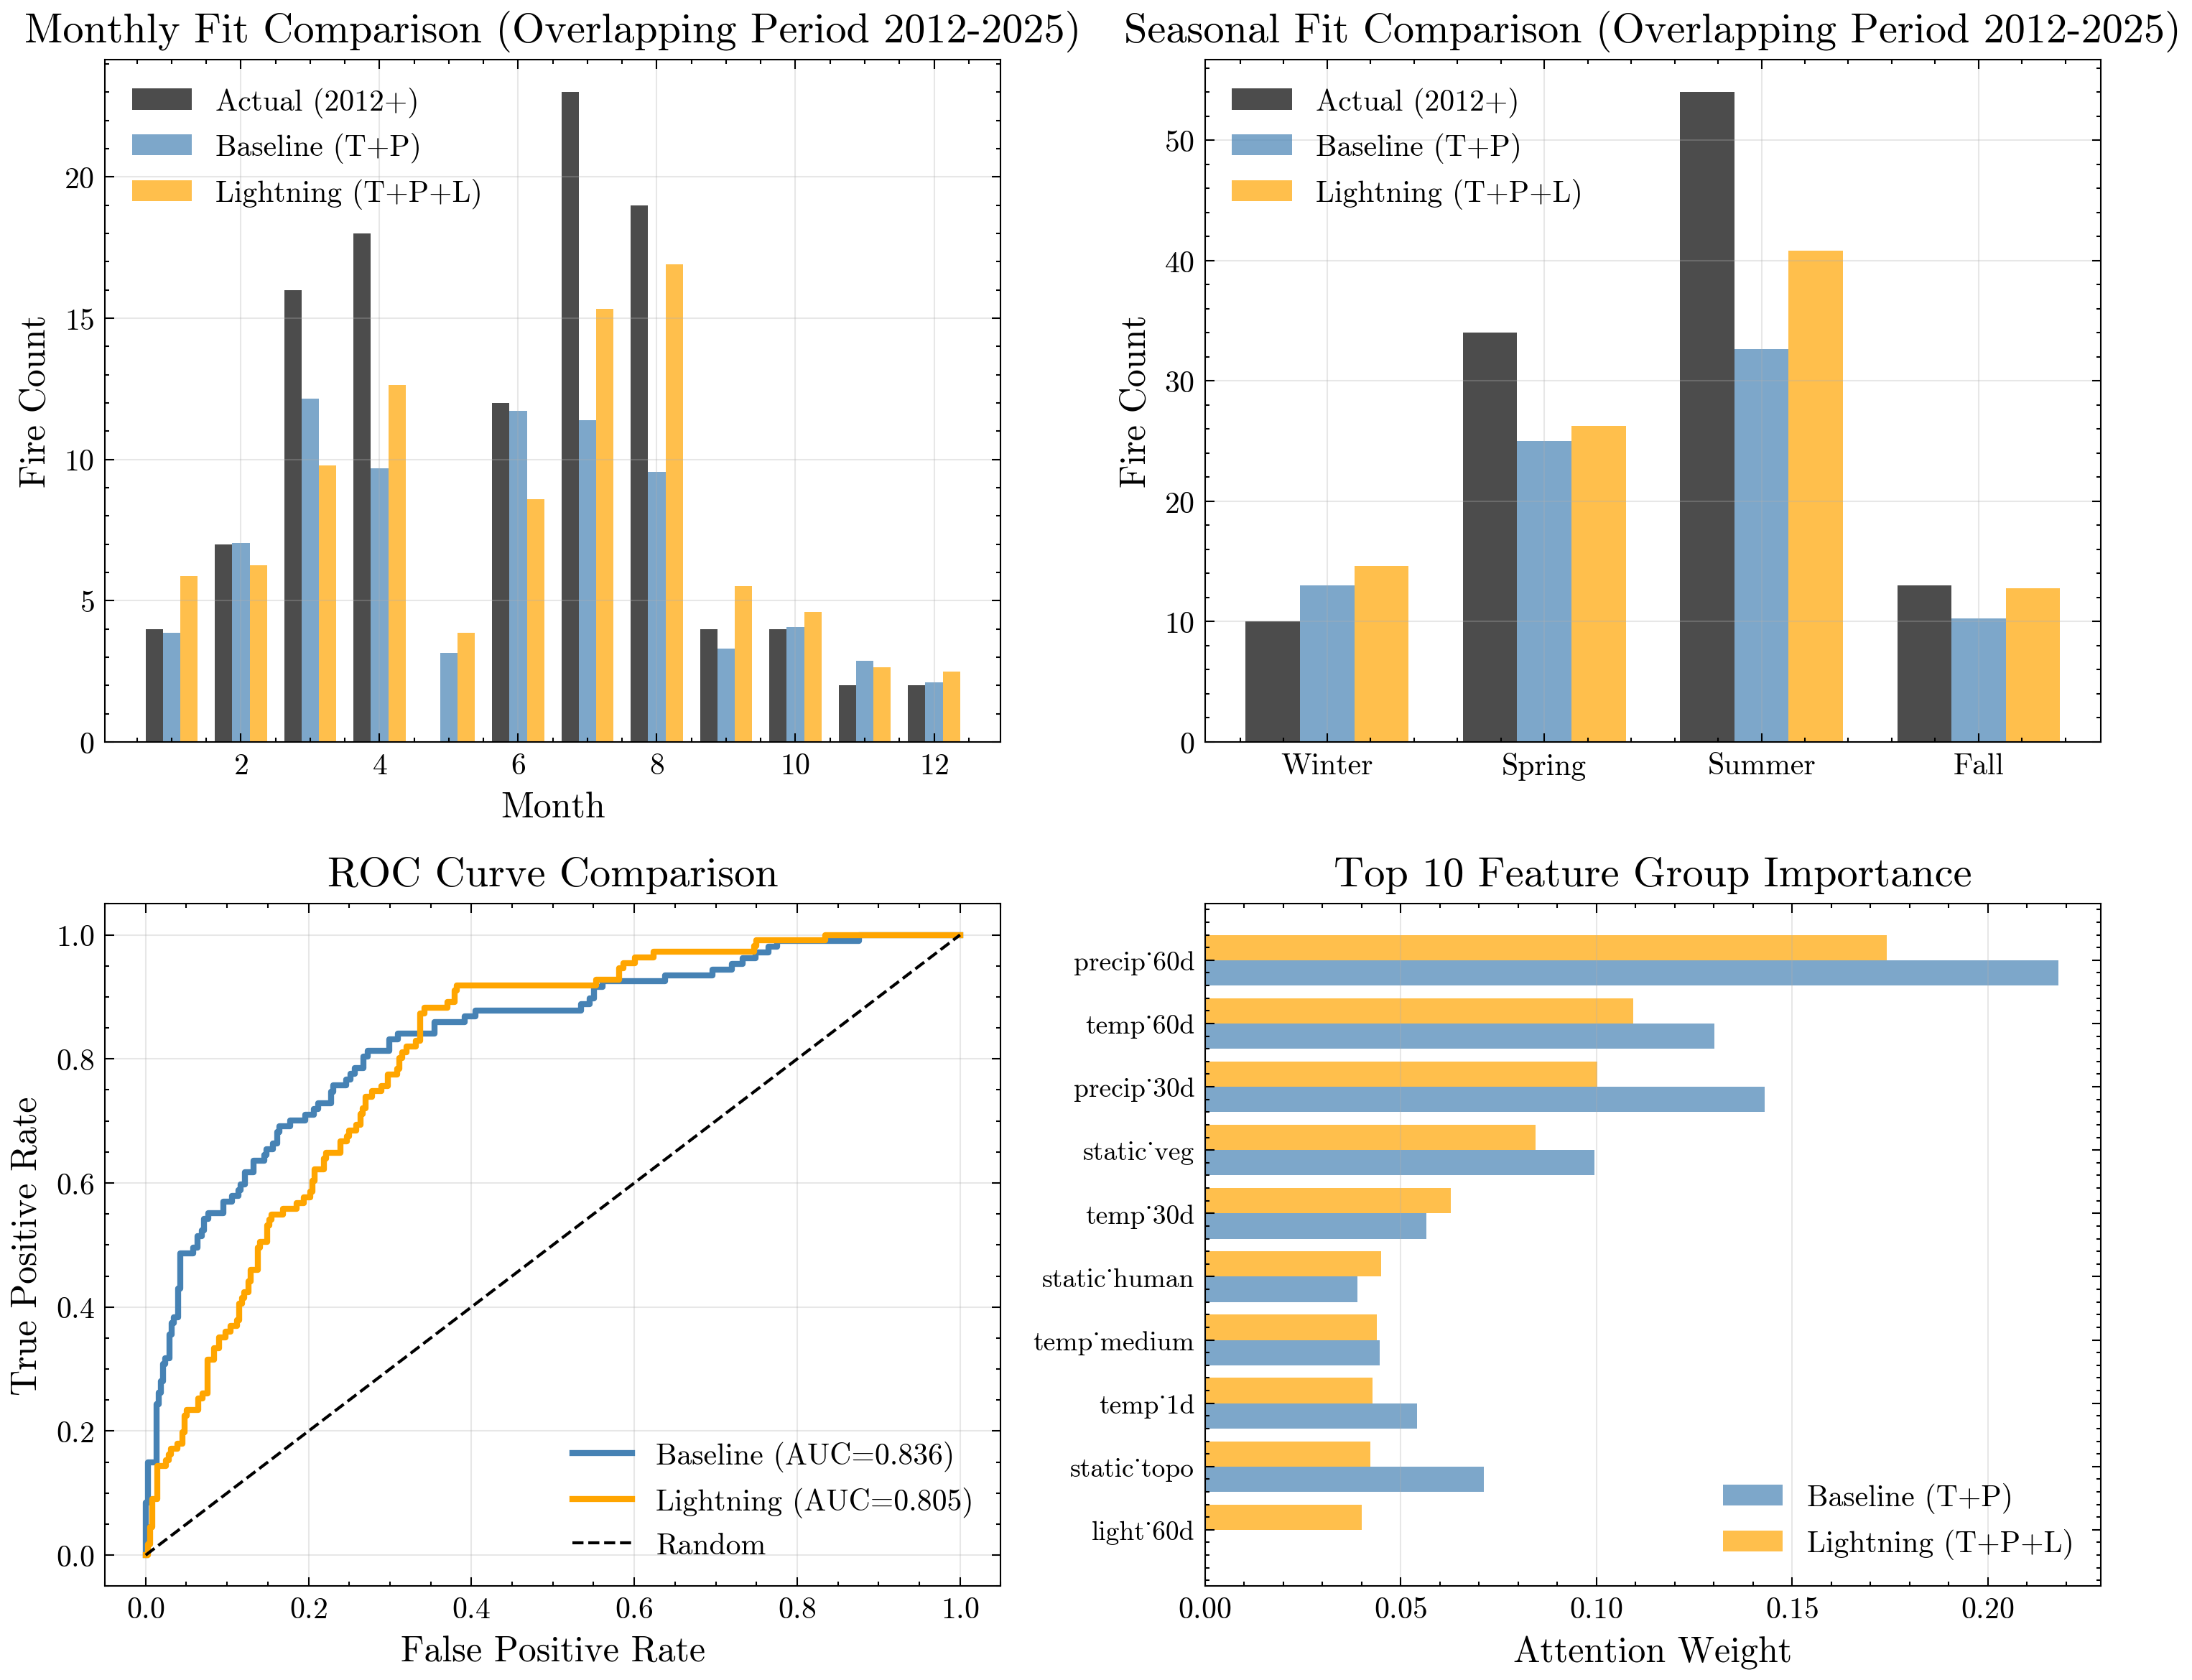
\includegraphics[width=\textwidth]{../output/figures/model_comparison.png}
\caption{Comprehensive model comparison: (top left) Monthly temporal fit showing superior performance of lightning model, (top right) ROC curves showing comparable discrimination with slight baseline advantage, (bottom left) Seasonal temporal fit with near-perfect lightning model performance, (bottom right) Feature importance via attention weights showing the contribution of different variable groups.}
\label{fig:model_comparison}
\end{figure}

\subsection{Feature Importance via Attention Weights}

The learned attention weights reveal the relative importance of different feature groups (Table \ref{tab:attention}).

\begin{table}[H]
\centering
\caption{Top feature groups by attention weight}
\label{tab:attention}
\begin{tabular}{llll}
\toprule
\textbf{Rank} & \textbf{Baseline Model} & \textbf{Lightning Model} & \textbf{Attention} \\
\midrule
1 & precip\_60d & precip\_60d & 0.218 / 0.174 \\
2 & precip\_30d & temp\_60d & 0.143 / 0.109 \\
3 & temp\_60d & precip\_30d & 0.130 / 0.100 \\
4 & static\_veg & static\_veg & 0.100 / 0.084 \\
5 & static\_topo & temp\_30d & 0.071 / 0.063 \\
\bottomrule
\end{tabular}
\end{table}

In the lightning model, lightning features collectively received attention weights of 0.174 distributed across temporal windows: light\_60d (0.040), light\_1d (0.036), light\_medium (0.034), light\_30d (0.033), light\_short (0.031).

\subsection{Climate Change Projections}

Using the baseline model, we projected future fire risk for Bolzano zones under RCP4.5 and RCP8.5 climate scenarios (Figure \ref{fig:climate_projections}).

\begin{figure}[H]
\centering
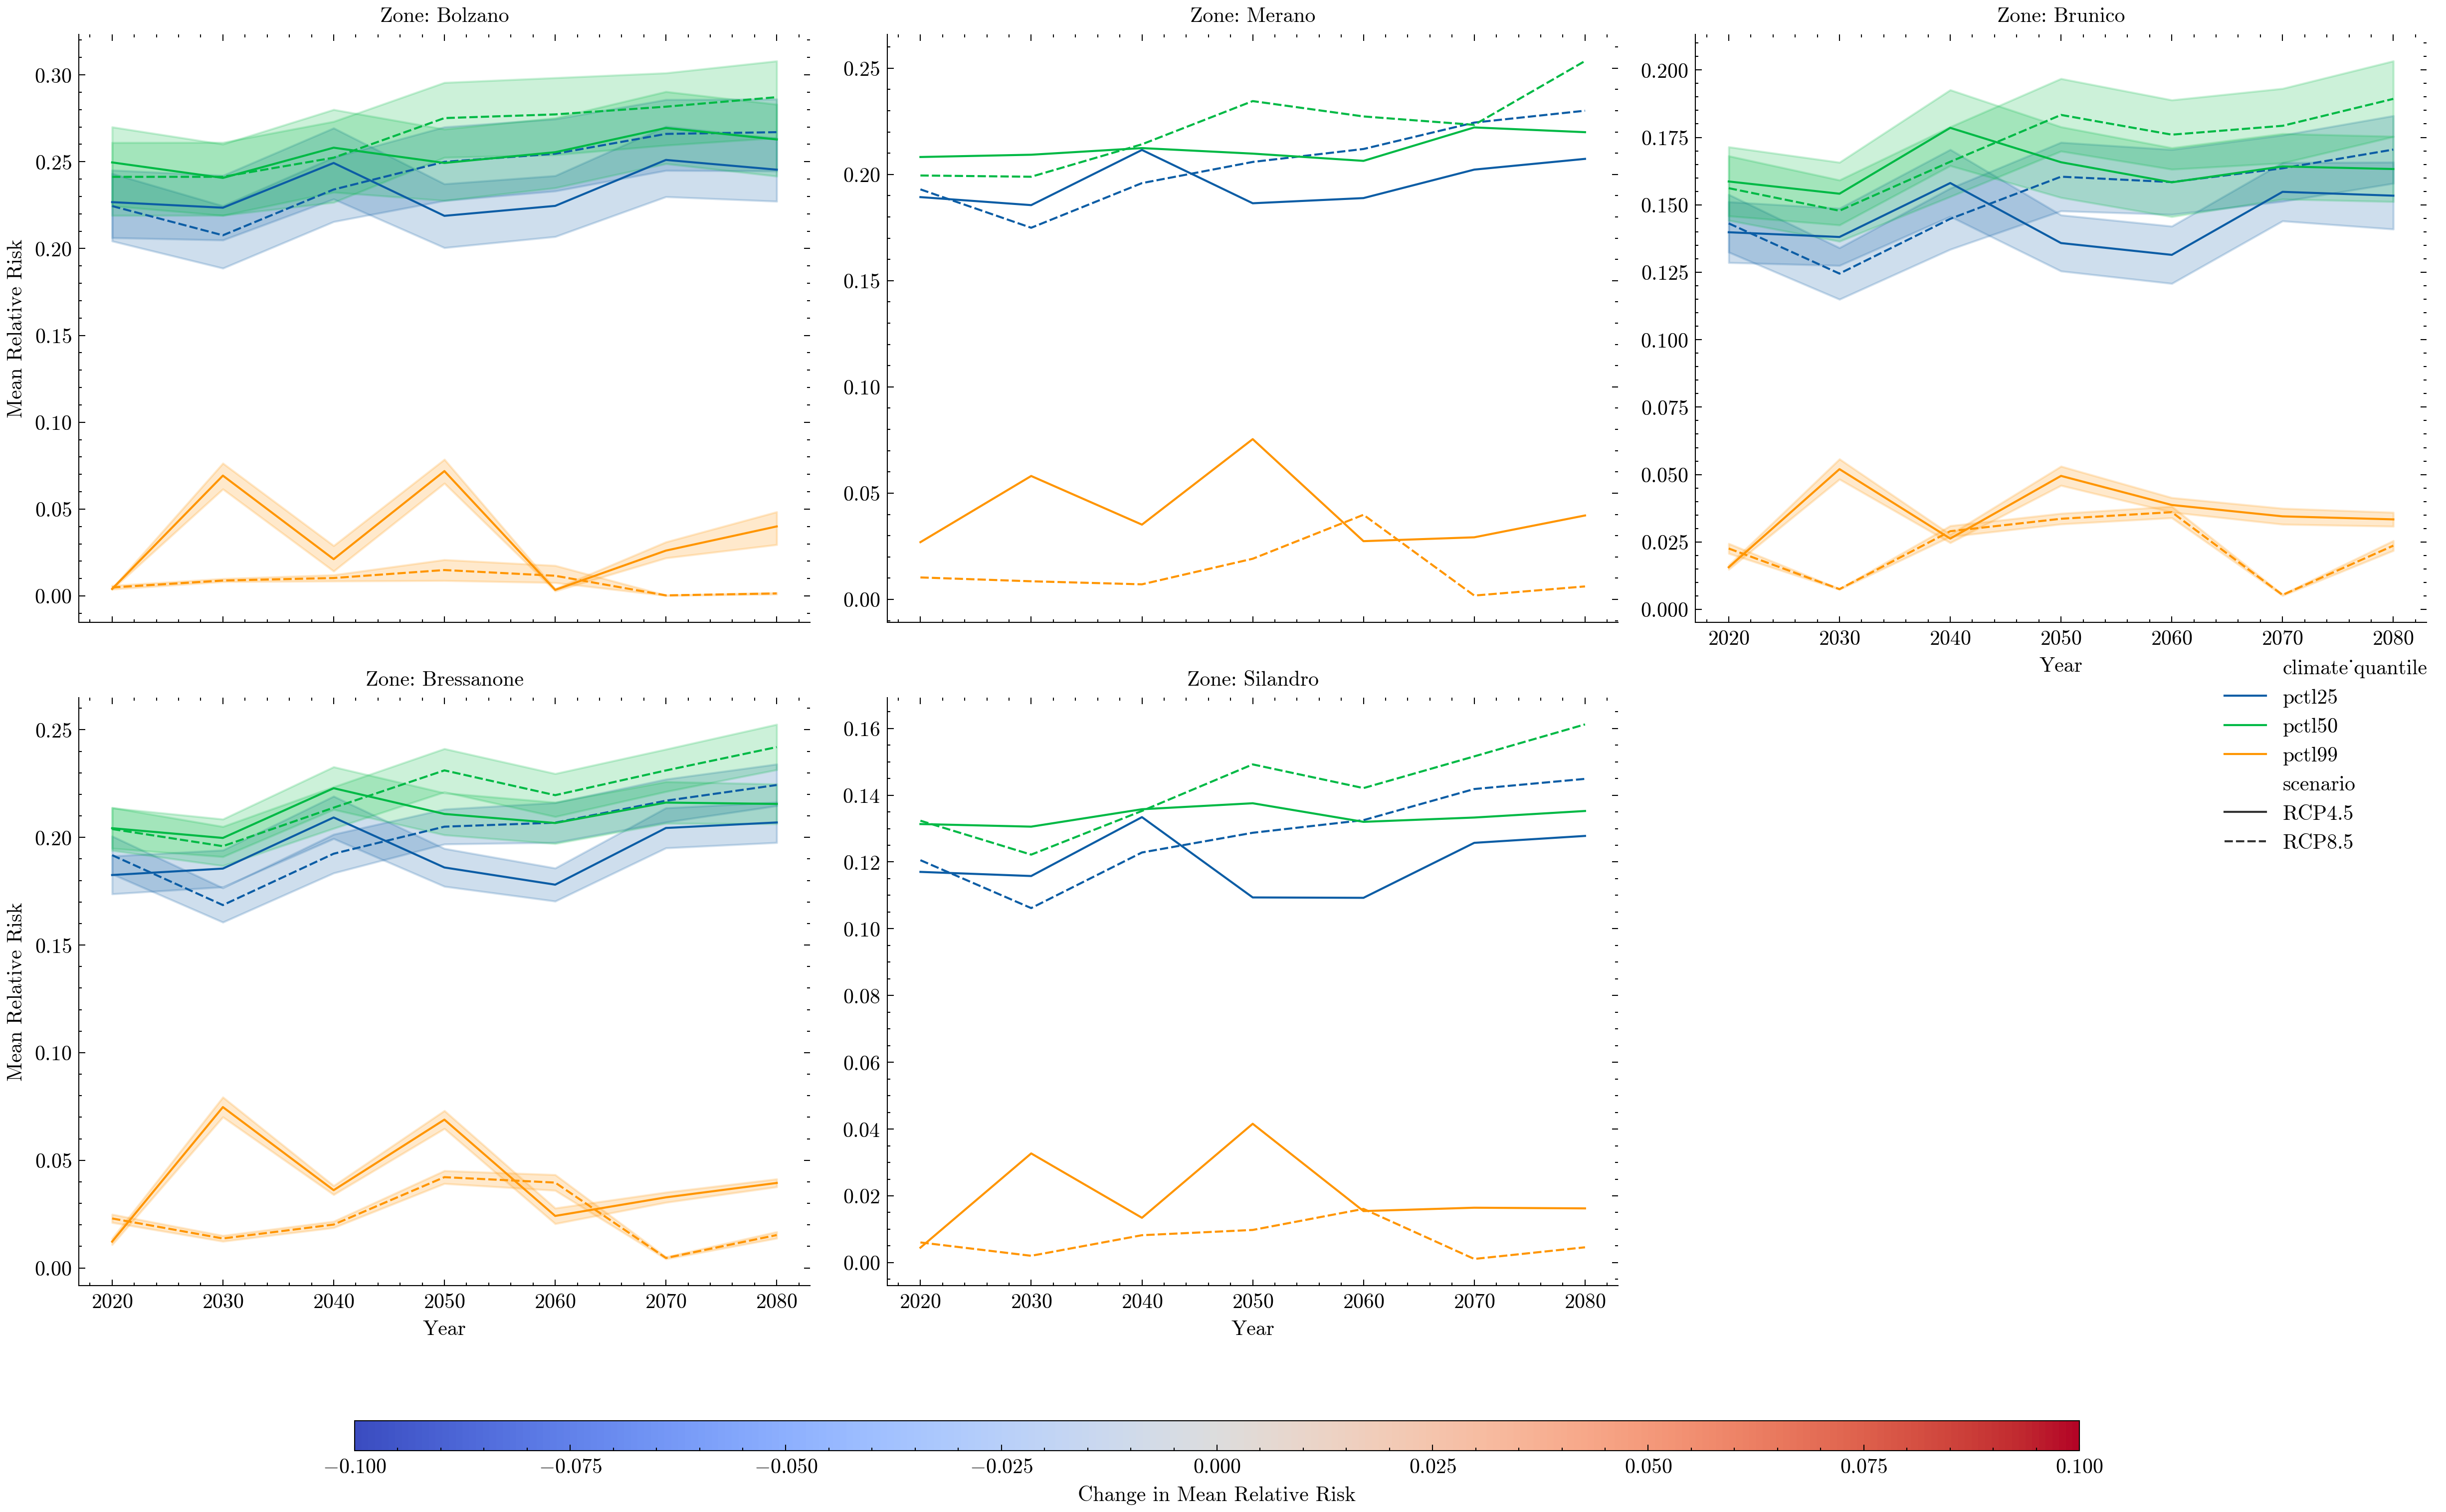
\includegraphics[width=0.48\textwidth]{../output/figures/climate_projection_plot_march.png}
\hfill
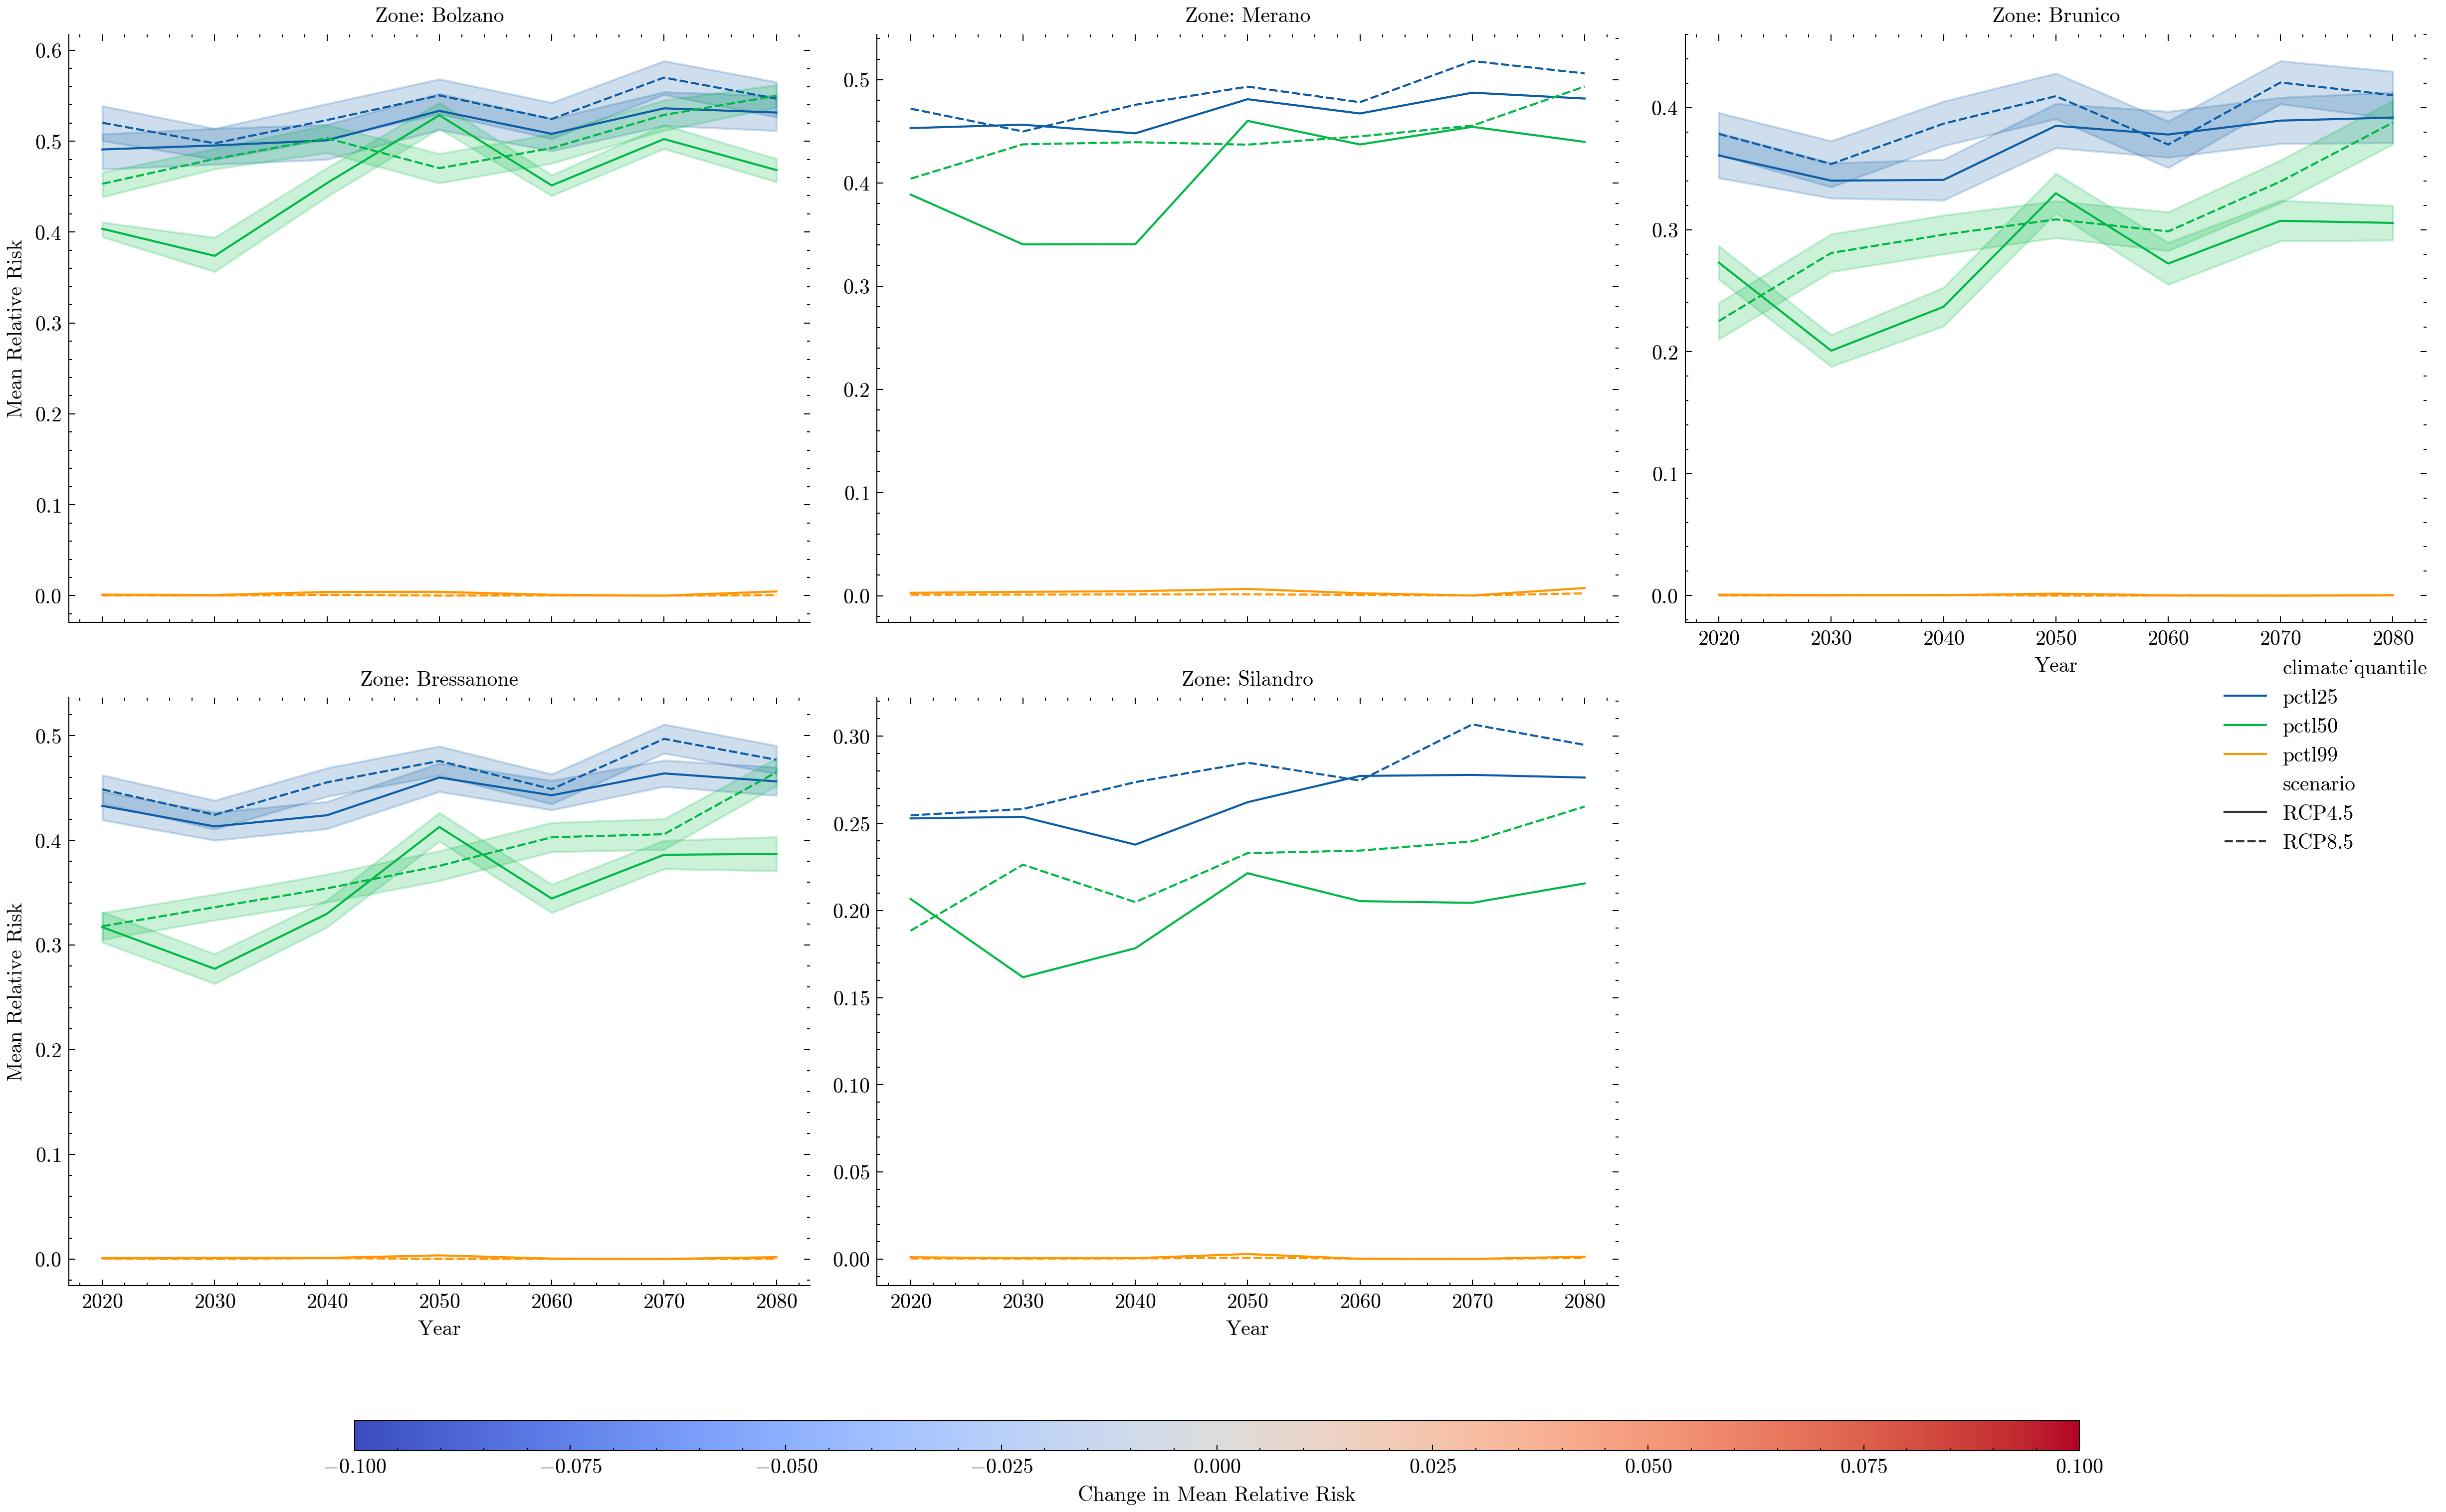
\includegraphics[width=0.48\textwidth]{../output/figures/climate_projection_plot_august.png}
\caption{Projected fire risk evolution for selected zones under RCP4.5 and RCP8.5 scenarios for March (left) and August (right). Lines show mean relative risk across different climate model quantiles, demonstrating increasing trend under both scenarios with greater uncertainty under RCP8.5.}
\label{fig:climate_projections}
\end{figure}

\section{Discussion}

\subsection{Complementary Model Strengths}

Our results reveal an interesting trade-off between temporal fidelity and spatial discrimination. The lightning-enhanced model dramatically improved temporal pattern prediction (+56\% seasonal R$^2$), making it ideal for applications requiring accurate forecasting of when fires are likely to occur---such as seasonal resource allocation, staffing decisions, and early warning systems.

Conversely, the baseline model maintained slightly better sample-level discrimination (+4\% ROC-AUC), suggesting advantages for applications focused on identifying high-risk locations at any given time---such as spatial prioritization of fuel treatments or infrastructure protection.

This finding has important operational implications: the optimal model choice depends on the primary management objective. For temporal forecasting (when), integrate lightning data. For spatial mapping (where), the simpler baseline may suffice or even outperform.

\subsection{Mechanisms of Lightning Contribution}

The strong improvement in temporal fit with lightning data likely reflects several mechanisms:

\begin{enumerate}
    \item \textbf{Direct ignition}: Lightning provides immediate ignition sources, creating sharp temporal signals
    \item \textbf{Seasonal proxy}: Lightning activity correlates with convective weather patterns that also promote fire spread
    \item \textbf{Elevation effects}: Lightning is particularly important at higher elevations where human ignitions are rare
\end{enumerate}

The attention weights show lightning features collectively receiving substantial importance (17.4\% total), particularly at longer temporal windows (60-day: 4\%), suggesting cumulative effects rather than just immediate ignition.

\subsection{Bayesian Framework Advantages}

The Bayesian approach provided several key advantages over traditional machine learning:

\begin{enumerate}
    \item \textbf{Uncertainty quantification}: Full posterior distributions enable probabilistic risk statements
    \item \textbf{Interpretability}: Hierarchical structure with attention weights reveals which features drive predictions
    \item \textbf{Calibration}: Posterior predictive checks ensure well-calibrated probability estimates
    \item \textbf{Small sample robustness}: Regularization via priors prevents overfitting despite limited lightning-era data (467 samples)
\end{enumerate}

\subsection{Operational Implications}

\subsubsection{Seasonal Planning}
The lightning model's near-perfect seasonal correlation (R$^2$=1.00) enables confident planning of seasonal resource allocation, staffing levels, and fuel treatment schedules months in advance.

\subsubsection{Early Warning Systems}
Real-time lightning detection integrated with the model could provide 24--48 hour fire risk forecasts with quantified uncertainty, allowing managers to adjust response levels and public communications.

\subsubsection{Resource Allocation}
The complementary strengths suggest a two-model approach: use lightning model for temporal forecasting and baseline model for spatial prioritization within forecast periods.

\subsection{Limitations and Future Directions}

\subsubsection{Data Limitations}
\begin{itemize}
    \item Lightning data limited to 2012--2025, preventing analysis of longer-term trends
    \item Spatial resolution (50m) may miss fine-scale fuel-topography interactions
    \item Human ignition patterns remain incompletely characterized
\end{itemize}

\subsubsection{Model Limitations}
\begin{itemize}
    \item Trade-off between temporal and spatial performance not fully understood mechanistically
    \item Relative probability outputs require additional calibration for absolute fire count prediction
    \item Climate projection uncertainty not fully propagated through the modeling chain
\end{itemize}

\subsubsection{Future Research}
\begin{enumerate}
    \item Extend lightning records through historical reconstruction or proxy data
    \item Develop hybrid models that optimize both temporal and spatial performance
    \item Integrate elevation-specific models given strong lightning-elevation relationships
    \item Couple fire-vegetation feedback for long-term projections
    \item Implement real-time operational systems with continuous model updating
\end{enumerate}

\section{Conclusions}

This study demonstrates that integrating lightning flash density data into Bayesian wildfire models substantially improves temporal prediction in Alpine environments, with monthly R$^2$ increasing from 0.77 to 0.93 and seasonal R$^2$ from 0.64 to 1.00. This enhancement comes with a minor trade-off in sample-level discrimination performance, revealing complementary strengths of the two modeling approaches.

Key findings include:

\begin{enumerate}
    \item \textbf{Lightning dramatically improves temporal fidelity} while maintaining reasonable spatial discrimination, making it valuable for seasonal forecasting and resource planning
    \item \textbf{Model choice depends on management objectives}: temporal forecasting favors lightning integration, spatial mapping may favor baseline approach
    \item \textbf{Bayesian framework provides essential uncertainty quantification} enabling risk-aware decision making
    \item \textbf{Attention mechanism reveals interpretable feature importance} showing precipitation (60-day), temperature (60-day), and lightning (collective) as key drivers
\end{enumerate}

Management implications:
\begin{itemize}
    \item Implement lightning-aware early warning systems for temporal forecasting
    \item Consider two-model approach: lightning for temporal, baseline for spatial prioritization
    \item Use uncertainty estimates for scenario planning and risk communication
    \item Expand lightning detection networks given demonstrated predictive value
\end{itemize}

As Alpine fire regimes continue evolving under climate change, probabilistic modeling frameworks that integrate diverse data streams and quantify uncertainty will become increasingly essential for sustainable forest management and civil protection in mountain environments.

% Acknowledgments
\section*{Acknowledgments}
We thank the Bolzano Forest Service Department for providing wildfire and operational data, and the South Tyrolean Civil Protection Agency for lightning detection records.

% Data Availability Statement
\section*{Data Availability}
Code and analysis workflows are available at: \url{https://github.com/alexandredunant/FireScape}. Processed datasets available upon request due to size constraints.

% References
\bibliographystyle{apalike}
\begin{thebibliography}{99}

\bibitem[Conedera et al., 2006]{Conedera2006}
Conedera, M., Cesti, G., Pezzatti, G.B., Zumbrunnen, T., and Spinedi, F. (2006).
\newblock Lightning-induced fires in the Alpine region: An increasing problem.
\newblock In \textit{Forest Fire Research}, pages 1--9.

\bibitem[Conedera et al., 2018]{Conedera2018}
Conedera, M., Krebs, P., Valese, E., et al. (2018).
\newblock Characterizing Alpine pyrogeography from fire statistics.
\newblock \textit{Applied Geography}, 98:87--99.

\bibitem[Kruschke, 2015]{Kruschke2015}
Kruschke, J.K. (2015).
\newblock \textit{Doing Bayesian Data Analysis: A Tutorial with R, JAGS, and Stan}.
\newblock Academic Press, 2nd edition.

\bibitem[Seidl et al., 2017]{Seidl2017}
Seidl, R., Thom, D., Kautz, M., et al. (2017).
\newblock Forest disturbances under climate change.
\newblock \textit{Nature Climate Change}, 7:395--402.

\end{thebibliography}

% Appendix
\appendix

\section{Model Implementation Workflow}

Figure \ref{fig:workflow} shows the complete data processing and modeling workflow used in this study.

\begin{figure}[H]
\centering
\tikzstyle{data} = [rectangle, rounded corners, draw=black, fill=gray!15,
                    text width=3.5cm, minimum height=1cm, text centered]
\tikzstyle{process} = [rectangle, draw=black, fill=blue!10,
                       text width=4cm, minimum height=1cm, text centered]
\tikzstyle{output} = [rectangle, draw=black, fill=green!15,
                      text width=3.5cm, minimum height=1cm, text centered]
\tikzstyle{arrow} = [thick, -{Latex[length=3mm, width=2mm]}]

\begin{tikzpicture}[node distance=1.5cm]

    % Inputs
    \node (input1) [data] {Meteorological Data \\ (precipitation, temperature)};
    \node (input2) [data, below=of input1] {Lightning Data \\ (flash density, 2012--2025)};
    \node (input3) [data, below=of input2] {Topographic \& Land Cover \\ (DEM, vegetation, roads)};
    \node (input4) [data, below=of input3] {Wildfire Inventory \\ (998 events, 1999--2025)};

    % Pre-processing
    \node (preproc) [process, right=3.5cm of input2.east] {Spatiotemporal Datacube \\ \small (32×32 pixels, 60-day lookback)};

    % Feature engineering
    \node (features) [process, below=of preproc] {Feature Engineering \\ \small (static, temporal, attention groups)};

    % Modelling step
    \node (model) [process, right=3.5cm of preproc] {Bayesian Hierarchical Model \\ \small (attention mechanism, MCMC)};

    % Parameters
    \node (param) [data, above=of model] {Priors \& Hyperparameters \\ \small (weakly informative)};

    % Outputs
    \node (output1) [output, right=3.5cm of model] {Relative Probability \\ (posterior distributions)};
    \node (output2) [output, below=of output1] {Uncertainty Estimates \\ (credible intervals)};
    \node (output3) [output, below=of output2] {Feature Importance \\ (attention weights)};

    % Arrows
    \draw [arrow] (input1) -- (preproc);
    \draw [arrow] (input2) -- (preproc);
    \draw [arrow] (input3) -- (preproc);
    \draw [arrow] (input4) -- (preproc);
    \draw [arrow] (preproc) -- (features);
    \draw [arrow] (features) -- (model);
    \draw [arrow] (param) -- (model);
    \draw [arrow] (model) -- (output1);
    \draw [arrow] (model) -- (output2);
    \draw [arrow] (model) -- (output3);

\end{tikzpicture}

\caption{Complete modeling workflow from raw data to outputs. The Bayesian hierarchical model with attention mechanism takes spatiotemporal datacubes and produces relative probability estimates with full uncertainty quantification.}
\label{fig:workflow}
\end{figure}

\end{document}
